\documentclass[bachelor,german]{mathe1thesis}

%\usepackage[utf8]{inputenc}
%\usepackage[T1]{fontenc}
\usepackage{fontspec}
\usepackage{wrapfig}
\usepackage{listings}

%\usepackage{lmodern} TODO: braucht man das?

\usepackage{tabularx}
\usepackage{ltablex}


\usepackage{path}
\usepackage{color}
\usepackage{dsfont}

\usepackage[disable,colorinlistoftodos]{luatodonotes}

\usepackage{xcolor}
\usepackage{float}
\usepackage{nameref}
\usepackage{algorithm2e} %for psuedo code


\definecolor{codegreen}{rgb}{0,0.6,0}
\definecolor{codegray}{rgb}{0.5,0.5,0.5}
\definecolor{codepurple}{rgb}{0.58,0,0.82}
\definecolor{backcolour}{rgb}{0.95,0.95,0.92}

\lstdefinestyle{mystyle}{
	backgroundcolor=\color{backcolour},   
	commentstyle=\color{codegreen},
	keywordstyle=\color{magenta},
	numberstyle=\tiny\color{codegray},
	stringstyle=\color{codepurple},
	basicstyle=\ttfamily\footnotesize,
	breakatwhitespace=false,         
	breaklines=true,                 
	captionpos=b,                    
	keepspaces=true,                 
	numbers=left,                    
	numbersep=5pt,                  
	showspaces=false,                
	showstringspaces=false,
	showtabs=false,                  
	tabsize=2
}

\lstset{style=mystyle}

% new operators
\DeclareMathOperator*{\argmax}{argmax}
\DeclareMathOperator*{\argmin}{argmin}
\DeclareMathOperator{\sign}{sign}
\DeclareMathOperator{\tf}{tf}


%%%%%%%%%%%%%%%%%%%%%%%%%%%%%%%%%%%%%%%%%%%%%%%%%%%%%%%%%%%%%%%%%%%%%%%%%%%%%%%%
%%% Titelseite -- hier Titel und Autorennamen eintragen
\title{Eine duale Koordinatenabstiegsmethode als SVM-Verfahren zur algorithmischen Umsetzung der automatischen Textklassifizierung} % Geben Sie hier den Titel Ihrer Arbeit an.
\subtitle{am Lehrstuhl für Mathematik VII}
\author{Simon Puglisi} % Geben Sie Ihren Namen an.
%\date{Eingereicht am \abgabedatum}
\titlehead{Julius-Maximilians-Universität Würzburg\\
Institut für Mathematik\\
Lehrstuhl für Mathematik VII\\
Numerische Mathematik und Optimierung}
\supervisors{Prof.\ Dr.\ Christian Kanzow}

\begin{document}
%%%%%%%%%%%%%%%%%%%%%%%%%%%%%%%%%%%%%%%%%%%%%%%%%%%%%%%%%%%%%%%%%%%%%%%%%%
%%%%%%%%%%%%% Bitte nur ab hier Änderungen vornehmen %%%%%%%%%%%%%%%%%%%%%

\begin{abstract}
    Die vorliegende Arbeit besteht aus fünf Teilen. Im ersten Kapitel befassen wir uns mit Klassifizierungsproblemen und Support-Vector-Machines (SVMs). Im zweiten Teil leiten wir mit einem anschaulichem topologischem Argument zwei hinreichende Konvergenzkriterien her. Im dritten Kapitel arbeiten wir eine Implementierung der L1/L2-Soft-SVM nach \cite{hcl-ddms-08} aus. Das nächste Kapitel stellt einen Kontext zur SVM und der Aufgabe der Textklassifizierung her. Zuletzt zeigen wir drei Experimente.

%    \vspace{3em}
%    \textbf{TODOs für die Titelseite:}
%    \todo{Soll der Name des Lehrstuhls für englische Arbeiten übersetzt werden?}
\end{abstract}

\thesistableofcontents


%%%%%%%%%%%%%%%%%%%%%%%%%%%%%%%%%%%%%%%%%%%%%%%%%%%%%%%%%%%%%%%%%%%%%%%%%%%%%%%%





%%%%%%%%%%%%%%%%%%%%%%%%%%%%%%%%%%%%%%%%%%%%%%%%%%%%%%%%%%%%%%%%%%%%%%%%%%%%%%%%




\chapter{Automatische Klassifizierung und Support Vector Machines}
Die Aufgabe der \emph{automatischen Klassifizierung} ist es, eine deterministische Funktion (oder ein Klassifikator beziehungsweise ein Klassifikationsverfahren) $f(x)$ anhand von \emph{Trainingsdaten} zu finden, die gewissen Daten $x \in \mathcal{X}$ eine (zu den Daten charakteristische) Klasse $y \in \mathcal{Y}$ zuweist. Verfahren dieser Art bezeichnen wir als \emph{(Lern-)Maschine} (\cite{b-tut-1998}). Die \emph{Support-Vector-Machine} (SVM) ist eine spezielle Lern-Maschine, die gewisse \glqq gute\grqq{} Eigenschaften besitzt, siehe hierzu \cite{b-tut-1998}. \\

Im folgenden Unterkapitel werden wir ein für uns geeignetes mathematisches Modell für die automatische Klassifizierung formulieren. Die SV-Machine behandeln wir im nächsten Unterkapitel.

\section{Automatische Klassifizierung}
Für die \emph{Textklassifizierung}, die wir später noch einführen werden, sind drei Typen von Klassifikatoren wesentlich.

\begin{definition}[Binär-Klassifikator]
	Sei $L=\{-1,1\}$ die Menge aller Klassen. Unter einem \emph{Binär-Klassifikator} verstehen wir eine Funktion $h:\mathbb{R}^n \rightarrow L$, die einem Datenvektor eine Klasse zuweist.
\end{definition}

\begin{definition}[Multi-Label-Klassifikator] \label{def:mlk}
	Sei $L=\{0 , 1 , 2 , ... , k\}$ die Menge aller Klassen. Unter einem \emph{Multi-Label-Klassifikator} (MLK) verstehen wir eine Funktion $h:\mathbb{R}^n \rightarrow  \mathcal{P}(L)$, die einen Datenvektor auf eine Menge Klassen zuweist. Die Menge $\mathcal{P}(L)$ bezeichnet die Potenzmenge von $L$.
\end{definition}

\begin{definition}[Multi-Klassen-Klassifikator]
	Sei $L=\{1 , 2 , ... , k\}$ die Menge aller Klassen. Unter einem \emph{Multi-Klassen-Klassifikator} (MKK) verstehen wir eine Funktion $h:\mathbb{R}^n \rightarrow  L$, die einen Datenvektor genau eine Klasse zuweist. 
\end{definition}

\begin{algorithm}[bhtp]
\KwIn{$x \in \mathbb{R}^n$}
\KwOut{$A \subset L$}
\KwData{Binärklassifikatoren $h_1,...,h_l$ bezüglich der einzelnen Klassen $1,...,l$}
$A \gets \{ \; \}$ \;
\ForEach{$i \in L$}{
	\If{$h_i(x) = 1$}{
		$A \gets A \cup \{i\}$
	}
}
\caption{Ein aus Binär-Klassifikatoren konstruierter MLK.}
\label{alg:mlk}
\end{algorithm}

Der Multi-Label-Klassifikator ist bei der Textklassifizierung nützlich, da die Textdokumente durchaus mehreren Themen zugeordnet werden können. Wie in Algorithmus \ref{alg:mlk} dargestellt lässt sich jeder MLK durch Binärklassifikatoren darstellen. Wir werden in Experiment C (Abschnitt \ref{sec:exp-c}) jedoch auf einen MKK zurückgreifen. Auch der MKK kann in vielen Fällen - und so auch bei der SVM - mit der \emph{one-vs-rest} Strategie (siehe \cite{hsu-comp-02}) über Binärklassifikatoren gewonnen werden. Aus diesem Grund wollen wir uns zunächst auf die Binärklassifikatoren beschränken. Im Abschnitt \nameref{sec:ovr} (Unterkapitel \ref{sec:ovr}) werden wir dann auf die Konstruktion eines MKKs genauer eingehen. Wir können also von folgendem Setting ausgehen: \\

Seien $(x^1,y^1),(x^2,y^2),...,(x^l,y^l)$ Trainingsdaten, wobei $x^i \in \mathbb{R}^n$  und $y^i \in \{-1,1\}$ die entsprechende Klasse für $1 \leq i \leq l$ sind. Wir werden wir immer fordern, dass $n\geq 2,\ x^i \neq 0$, sowie $y^i \neq y^j$ für alle  $1 \leq i \leq l$ und mindestens ein $j,\  1 \leq j \leq l$ gelten. \\


Eine Qualitätsgröße für einen Klassifikators liefert uns das \emph{empirische Risiko}:
\begin{definition}[Empirisches Risiko]
	Sei $h: \mathbb{R}^n \rightarrow \{-1,1\}$. Dann ist das empirische Risiko definiert durch
	\begin{equation}
	R_{emp}(h) := \frac{1}{l} \cdot \sum_{i=1}^{l}{\mathds{1}_{\{ h \neq y^i \}}(x^i)},
	\end{equation}
	wobei mit $\mathds{1}_{A}$ die \emph{Indikatorfunktion} gemeint ist und die Menge $A=\{ h \neq y^i \}=\{ x \in \mathbb{R}^n \ | \ h(x) \neq y^i \}$ gesetzt wurde. 
\end{definition}

Das empirische Risiko schätzt also den zu erwartenden Fehler bei Anwendung des Klassifikationsverfahrens. Wir werden später illustrieren, dass das empirische Risiko alleine nicht unbedingt ein vertrauensvolle Größe für die Abschätzung der \emph{Generalisierungsfähigkeit} eines Klassifikators ist. Nach \cite{sb-umlfta} lässt sich eine höhere Generalisierungsfähigkeit hingegen durch bestimmte einschränkende Bedingungen an die zu betrachtende Funktionsklasse $\mathbb{H} \subset \{ \, h \, \mid  \, h: \mathbb{R}^n \rightarrow \{-1 ,\ 1\} \, \}$ bewerkstelligen. Hat man eine Funktionsklasse $\mathbb{H}$ gegeben, so kann eine Lern-Maschine beispielsweise den Klassifikator aus $\mathbb{H}$ auswählen, der das empirische Risiko bezüglich der gegebenen Trainingsdaten minimiert.

\begin{definition}[Empirische Risikominimierung]
	\label{definition-erm}
	Sei $\mathbb{H} \subset \{ \, h \, \mid  \, h: \mathbb{R}^n \rightarrow \{-1 ,\ 1\} \, \}$.
	Wir bezeichnen das Problem
	\begin{equation}
	\label{equ-erm}
	h^*(x) := \argmin_{h \in \mathbb{H}} R_{emp}(h)
	\end{equation}
	als \emph{empirische Risikominimierung} bezüglich $\mathbb{H}$. Hat  (\ref{equ-erm}) eine Lösung $h^*$, so bezeichnen wir mit $h^*$ einen optimalen Klassifikator (bezüglich $\mathbb{H}$).
\end{definition}

Die empirische Risikominimierung kann uns also eine Anleitung für die Konstruktion einer Lernmaschine liefern. 

\section{Lineare Klassifikatoren}
Eine einfache Funktionsklasse, die bei bestimmten Problemen durchaus Anwendung findet, ist die Klasse der \emph{linearen Klassifikatoren} (Definition \ref{def-lin-klass}). Diese doch starke Einschränkung wirkt sich im Allgemeinen sicherlich nicht minimierend auf das empirische Risiko aus. Auf der anderen Seite kann die Einschränkung jedoch für eine höhere Generalisierungsfähigkeit hilfreich sein, siehe hierzu \cite{sb-umlfta}. Wir wollen die \glqq linearen Klassifikatoren\grqq{} nun mathematisch formulieren. Hierfür werden wir zunächst ein paar Definitionen einführen.

\begin{definition}[Hyperebene]
	\label{def-hyperebene}
	Seien $(w,b) \in \mathbb{R}^n \times \mathbb{R}$. Wir nennen die Menge
	\begin{equation}
		\label{hyperebene}
		E_{(w,b)}=\{ x \in \mathbb{R}^n \mid w^tx + b = 0 \}
	\end{equation}
	\emph{Hyperebene} im Raum $\mathbb{R}^n$ bezüglich $(w,b)$. Oft werden wir auch von der Hyperebene $(w,b)$ sprechen, wobei immer die durch $(w,b)$ induzierte Menge (\ref{hyperebene}) gemeint ist.
\end{definition}

\begin{definition}[Abstand zur Hyperebene]
	Seien $x \in \mathbb{R}^n, \ (w,b) \in \mathbb{R}^n \times \mathbb{R}$. Dann ist 
	der Abstand von $x$ zur Hyperebene $E_{(w,b)}$ durch
	\begin{equation}
		d(E_{(w,b)},x) := \inf_{y \in E_{(w,b)}} ||y-x||
	\end{equation}
	definiert.
\end{definition}

\begin{lemma}
	\label{lemma-abstand-norm}
	Seien $x \in \mathbb{R}^n, \ (w,b) \in \mathbb{R}^n \times \mathbb{R},\ ||w|| = 1$.
	Dann ist der \emph{Abstand} $d(E_{(w,b)},x)$ von $x$ zur Hyperebene $E_{(w,b)}$ durch $| \langle w,x \rangle +b |$ gegeben.
\end{lemma}
\begin{proof}
	Siehe hierzu beispielsweise den Beweis von Behauptung 15.1. in \cite{sb-umlfta}.
\end{proof}

\begin{lemma}
	\label{lemma-abst-hyp-allg}
	Seien $x \in \mathbb{R}^n, \ (w,b) \in \mathbb{R}^n \times \mathbb{R}$. 
	Dann ist der Abstand $d(E_{(w,b)},x)$ von $x$ zur Hyperebene $E_{(w,b)}$ durch
	$\frac{1}{||w||}|\langle w,x \rangle + b|$
	gegeben.
\end{lemma}
\begin{proof}
	Setze $\tilde{w} := \frac{w}{||w||}$ und $\tilde{b} := \frac{b}{||w||}$. Dann ist der Abstand zwischen $x$ und der Hyperebene $(\tilde{w},\hat{b})$ nach dem vorherigen Lemma
 	$\langle \tilde{w},x \rangle + \tilde{b} = \frac{1}{||w||}|\langle w,x \rangle + b|$. 
 	Da die Beziehung $E_{(w,b)}=E_{(\tilde{w},\tilde{b})}$ gilt, ist das Lemma bewiesen. 
\end{proof}

\begin{definition}[Lineare Separierbarkeit]
	\label{def-lin-sep}
	Wir sagen, die Vektoren $(x^1,y^1),...,(x^l,y^l)$ mit $x^i \in \mathbb{R}^n$  und $y^i \in \{-1,1\} ,\ 1 \leq i \leq l$ sind genau dann \emph{linear separierbar}, wenn eine Hyperebene $(w,b) \in \mathbb{R}^{n+1}$ existiert, sodass 
	\begin{equation}
		\label{equ-lin-sep}
		y^k(w^tx^k+b) > 0, \ \text{für alle} \ 1 \leq k \leq l
	\end{equation}
	gilt. Weiter sagen wir, $(w,b)$ separiert die Vektoren $(x^1,y^1),(x^2,y^2),...,(x^l,y^l)$ genau dann, wenn (\ref{equ-lin-sep}) gilt. Wir werden Separierbarkeit und lineare Separierbarkeit als Synonyme verwenden. 
\end{definition}

\begin{bemerkung}
	Die Bedingung (\ref{equ-lin-sep}) impliziert, dass der Abstand $d(E_{(w,b)},x^k)$ aller Datenvektoren 
	$x^k, \ \text{mit} \ 1 \leq k \leq l$ zur Hyperebene $E_{(w,b)}$ positiv $(> 0)$ sein muss. Weiter legt  (\ref{equ-lin-sep}) genau fest, in welchen der durch die Hyperebene induzierten Halbräumen die Vektoren liegen müssen.
\end{bemerkung}

Solange nicht anders erwähnt, setzen wir im Folgenden die lineare Separierbarkeit der Vektoren $(x^1,y^1),...,(x^l,y^l)$ immer voraus. 

\begin{definition}[Linearer Klassifikator]
	\label{def-lin-klass}
	Wir definieren mit
	\begin{equation}
	h_{(w,b)}(x) := \sign(w^t  x + b)
	\end{equation} 
	einen durch die Hyperebene $(w,b) \in \mathbb{R}^n \times \mathbb{R}$ induzierten \emph{linearen Klassifikator}.
\end{definition} 

Der lineare Klassifikator ist offenbar nur auf der Menge $\mathbb{R}^n \setminus E_{(w,b)}$ sinnvoll definiert. Für Datenvektoren innerhalb der Ebene kann in diesem Setting keine sinnvolle Entscheidung bezüglich der Klassenzugehörigkeit getroffen werden. Formal setzen wir in diesem Fall $h_{(w,b)}(x)=\infty$ und erweitern $L$ zu $\tilde{L}=\{ -1,\ 1,\ \infty \}$. Dies erlaubt uns die Menge der linearen Klassifikatoren in der kompakten Form 
\begin{equation}
	\label{equ-H}
	\mathbb{H} = \{ h_{(w,b)} \mid R_{emp}(h_{(w,b)}) = 0 \}
\end{equation}
zu schreiben. Offenbar besteht $\mathbb{H}$ aus genau jenen linearen Klassifikatoren, dessen korrespondierende Hyperebenen die Datenvektoren $(x^1,y^1),...,(x^l,y^l)$ separieren. Im Sinne der empirischen Risikominimierung ist also jeder lineare Klassifikator aus $\mathbb{H}$ optimal.  \\

\begin{figure}
	\begin{center}
		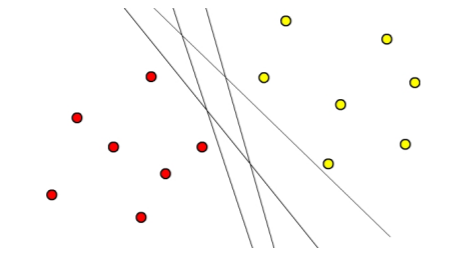
\includegraphics{abbildungen/trennungen.PNG}
	\end{center}
	\caption{Die Abbildung zeigt verschiedene trennende Ebenen für die gelben und roten Datenvektoren.}
	\label{pic-sep-hyp}
\end{figure}

Die Abbildung \ref{pic-sep-hyp} illustriert ein Klassifizierungsproblem bestehend aus roten und gelben Datenvektoren, sowie hierfür zulässige lineare Klassifikatoren im Sinne von (\ref{equ-H}). Das empirische Risiko liefert uns kein Indiz für einen möglichst generalisierenden Klassifikator. Zu erkennen sind jedoch Ebenen mit größeren und kleineren Abständen zu den roten oder gelben Datenvektoren. Im nächsten Unterkapitel werden wir diese Tatsache für die Konstruktion der SVM nutzen. \\

Der nächste Satz \ref{satz-svm-ls} zeigt uns, dass der Abstand der Hyperebenen aus $\mathbb{H}$ sogar beliebig klein zu den Trainingsvektoren beider Klassen werden kann. 
\begin{satz}
	\label{satz-svm-ls}
	Sei $\varepsilon > 0$. Dann existieren ein linearer Klassifikator $h_{(w,b)} \in \mathbb{H}$, sowie $i = 1,...,l,\ j = 1,...,l$ mit $y^i \neq y^j$, sodass $d(E_{(w,b)},x^i) < \varepsilon$ und $d(E_{(w,b)},x^j) < \varepsilon$ gelten.
\end{satz}
\begin{proof}
	Sei 
	\begin{equation}
	\begin{aligned} \label{min-prog-h}
		& \smash{\min_{\substack{(w,b) \\ ||w||=1 }} \; 
				d(E_{(w,b)},x^i) + d(E_{(w,b)},x^j)
		} \qquad \text{u.d.N.} 
		\qquad & y^k(w^tx^k+b) \geq 0 \\
			   && k = 1,...,l
	\end{aligned}
	\end{equation}
	ein Minimierungsproblem mit $y^i=1$ und $y^j=-1$ für $0 \leq i \le j \leq n$. Die Zielfunktion aus (\ref{min-prog-h}) lässt sich weiter zu 
	\[
		 d(E_{(w,b)},x^i) +d(E_{(w,b)},x^j) = y^i(w^t x^i+b) + y^j(w^t x^j +b) = w^t(x^i-x^j)
	\]
	vereinfachen. 
	Die Bedingung $||w||=1$ schließt $(w,b)=0$ als triviale Lösung von (\ref{min-prog-h}) aus. Aus der Separierbarkeit der Trainingsvektoren folgt, dass die zulässige Menge nicht leer ist. Weiter ist die zulässige Menge abgeschlossen. Die Beschränktheit kann man sich wie folgt klar machen: 
	
	Definiere 
	\begin{equation}\label{equ:bounded-set}
	M' := \max_{||w|| = 1}{\max_{1 \leq i \leq l}{y^i \langle w, x^i \rangle}}.
	\end{equation}
	Sei weiter $(w,b)$ für das Problem (\ref{min-prog-h}) zulässig. Wir wollen zeigen dass dann $|b|<M'$ gelten muss.
	Angenommen $b > M'$. Dann folgt mit (\ref{equ:bounded-set}) (und $y^j=-1$) die strikte Ungleichung 
	$$
	y^j(w^t x^i + b) = y^j w^t x^i - b < y^j w^t x^i  - M' \leq 0.
	$$
	Im Widerspruch zur Zulässigkeit von $(w,b)$. Die Annahme $b < M'$ führt zu einem analogen Widerspruch, sodass wir $|b| \leq M'$ fordern können. 
	Damit ist die zulässige Menge abgeschlossen und beschränkt,	nach dem Satz von Heine-Borel (vgl. \cite{ae-ana1}) also kompakt. Da außerdem die Zielfunktion stetig ist, sichert uns der Satz vom Minimum und Maximum  (vgl. \cite{ae-ana1}) die Existenz einer Lösung $(w_{i,j}^*,b_{i,j}^*)$ zum entsprechenden Minimum  $M_{(i,j)}$. 
	Da der Abstand stets nicht negativ ist, folgt $M_{(i,j)} \geq 0$. 
	
	Wir dürfen nach eventueller Umbenennung annehmen, dass $(i,j)$ so gewählt ist, dass die Gleichung 
	$$
	(i,j) = \argmin_{1\leq q,r \leq l} \; \{ M_{(q,r)} \mid (y^q,y^r)=(1,-1) \}
	$$ 
	erfüllt ist, wobei $M_{(q,r)}$ die entsprechenden Lösungen von (\ref{min-prog-h}) für $(q,r)$ sind. \\
	
	Seien nun $M := M_{(i,j)}$, sowie  $(w^*,b^*) := (w_{i,j}^*,b_{i,j}^*)$. Können wir zeigen, dass $M=0$ gilt, ist der Satz bewiesen.
	Um dies zu sehen sei $M=0$ und $(v,p)$ eine separierende Hyperebene der Trainingsdaten. Dann induziert für beliebiges $\beta > 0$ der Vektor $e(\beta) := (w^*,b)+ \beta (v,p)$ einen linearen Klassifikator, also ist $h_{e(\beta)} \in \mathbb{H}$. Jetzt folgt mit
	$$
	\begin{aligned}
	d(E_{e(\beta)},x^{i/j}) &= ((w^*)^t+\beta v^t) x^{i/j} + (b^*+\beta p) = (w^*)^t x^{i/j} + b^* + \beta (v^t x^{i/j} + p) = \\
	&= 0 + \beta (v^t x^{i/j} + p) \xrightarrow{\beta \rightarrow 0} 0
	\end{aligned}
	$$ 
	die Behauptung. \\
	
	Angenommen $M \neq 0$. Da dann $M>0$ gelten muss, ist $d(E_{(w^*,b^*)},x^i) > 0$ oder $d(E_{(w^*,b^*)},x^j) > 0$. \\
	
	Wir nehmen zunächst an, dass der Abstand der Ebene zu einem Datenvektor $0$ ist. O.b.d.A. sei $d(E_{(w^*,b^*)},x^i) = 0$. Den anderen Fall behandeln wir analog. Da dann wegen der Wahl von $(i,j)$
	$$
	d(E_{(w^*,b^*)},x^k) \geq d(E_{(w^*,b^*)},x^j) > 0
	$$ 
	für alle $k$ mit $y^k = -1$ gilt, existiert ein $\bar{b}>0$, dass mit $\bar{e} := (w^*, b^*+ \bar{b})$ der Abstand  $d(E_{\bar{e}}, x^k) > 0$ für alle $1 \leq k \leq n$ ist. Insbesondere ist $\bar{e}$ zulässig für (\ref{min-prog-h}). Weiter ist 
	$$
	d(E_{\bar{e}},x^i) + d(E_{\bar{e}},x^j) 
	 = (w^*)^t(x^i-x^j) 
     = d(E_{(w^*,b^*)},x^i) +d(E_{(w^*,b^*)},x^j),
	$$
	wobei die zweite Gleichheit aus  $y^i+y^j=0$ folgt. 
	Damit wäre $\bar{e}$ eine weitere Lösung des Problems (\ref{min-prog-h}) mit $M > 0$. \\
	
	Es reicht also den Fall $M>0,\ d(E_{(w^*,b^*)},x^i) > 0$ sowie $d(E_{(w^*,b^*)},x^j) > 0$ zu widerlegen. Wir wollen dies mit einem Widerspruch erreichen. Da also in diesem Fall keine der Nebenbedingungen aktiv ist, haben wir die Freiheit die linearen Restriktionen in einer hinreichend kleinen Umgebung von $w^*$ zu ignorieren. Wir suchen jetzt ein $\bar{w}$, sodass
	$$
		\begin{aligned}
		\bar{w}^t(x^i-x^j) &< (w^*)^t(x^i-x^j) \\
		     ||\bar{w}|| &= 1 \\
		 ||\bar{w}-w^*|| &< \delta
		\end{aligned}
	$$
	für ein beliebig klein gewähltes $\delta > 0$ gilt. Transformieren wir das Koordinatensystem über eine (isometrische) Drehung so um, dass $(x^i-x^j)=\eta e_n$ für ein positives $\eta$ gilt, erkennen wir, dass die n-te Komponente $w^*_n$ von $w^*$ wegen
	$$
	\eta w^*_n = (w^*)^t (x^i-x^j) = d(E_{(w^*,b^*)},x^i) + d(E_{(w^*,b^*)},x^j) = M > 0
	$$ 
	positiv sein muss. Wir sind also in der Situation, dass wir auf der Nordhalbkugel von $S^{n-1} := \{x \in \mathbb{R}^n \mid ||x|| = 1 \}$ nach einem $\bar{w}$ suchen, sodass $0 \leq \bar{w}_n < w_n^*$ gilt. Es ist ersichtlich, dass hierfür eine stetige Kurve $\gamma : [0,t_0] \rightarrow S^{n-1}$ mit $\gamma(0) = w^*$ und $ \gamma(t) < (w^*)^t(x^i-x^j)$ für $t \in (0, t_0]$ existiert. Wegen der Stetigkeit von $\gamma$ finden wir schließlich ein $t_1$, sodass mit $\bar{w} := \gamma(t_1)$ der Punkt $(\bar{w},b^*)$ zulässig für ($\ref{min-prog-h}$) ist. Nach obiger Argumentation wäre dann aber $0 \leq \bar{w}^t(x^i-x^j) < (w^*)^t(x^i-x^j) = M$, was nach Konstruktion von $M$ nicht möglich ist. Also muss $M=0$ gewesen sein.
	
\end{proof} 
 
\section{Support-Vector-Machines}
In \cite{sb-umlfta} stellt sich heraus, dass der Abstand der separierenden Hyperebenen eines linearen Klassifikators $h_{(w,b)} \in \mathbb{H}$ zu den Datenvektoren ein geeignetes Gütemaß für die Generalisierungsfähigkeit für $h_{(w,b)}$ ist. Dieser Sachverhalt motiviert die Support-Vector-Machine (SVM): Die SVM liefert den linearen Klassifikator $h^*_{(w^*,b^*)}$, dessen Hyperebene $E_{(w^*,b^*)}$ den Abstand zu den Datenvektoren $(x^1,...,x^l)$ maximiert. Die SVM lässt sich damit als das Optimierungsproblem
\begin{equation}
	\label{equ-svm-1}
	\begin{aligned}
	\argmax_{||w||=1} { \; \min_{1 \leq i \leq l}{ \; d(E_{(w,b)}, x^i) }} \qquad
					  \text{u.d.N.} \qquad h_{(w,b)} \in \mathbb{H}
 	\end{aligned}
\end{equation}
auffassen. In anderer Notation aufgeschrieben (siehe Lemma \ref{lemma-abstand-norm}, Definition \ref{def-lin-sep}, sowie Gleichung (\ref{equ-H})) ergibt dies
\begin{equation}
	\label{svm-min-max-nb}
	\begin{aligned}
		& \smash{ \argmax_{\substack{||w||=1 \\ (w,b) \in \mathbb{R}^n \times \mathbb{R}}}{ 
			\min_{1\leq i \leq l}{y^i(\langle w, x^i \rangle + b)}
		}} \qquad \text{u.d.N.} \qquad &
		y^i(\langle w, x^i \rangle + b) > 0 \\ 
		&& i = 1,...,l
	\end{aligned}
\end{equation}
Wir wollen nun zeigen, dass (\ref{equ-svm-1}) eine Lösung besitzt. Dies ist nicht unmittelbar klar, da $\mathbb{H}$, wie in Satz \ref{satz-svm-ls} zu sehen ist, nicht abgeschlossen ist (wenn man als Norm den Abstand der korrespondieren Ebenen heranzieht). Um die Lösbarkeit zu zeigen, werden wir (\ref{svm-min-max-nb}) geeignet umformulieren. Zunächst zeigen wir die Äquivalenz von (\ref{svm-min-max}) mit

\begin{equation}
\label{svm-min-max}
\begin{aligned}
	\argmax_{\substack{||w||=1 \\ (w,b) \in \mathbb{R}^n \times \mathbb{R}}}{
		\min_{1\leq i \leq l}{y^i(\langle w, x^i \rangle + b)}
	}.
\end{aligned}
\end{equation}

Anschließend führen wir die \emph{Hard-SVM} (Definition \ref{hard-svm}) ein. In Lemma \ref{lemma-svm-prob-aequ} ergibt sich schließlich die Äquivalenz aller drei Probleme. In Lemma \ref{lemma-hard-svm-loes} wird abschließend die Lösbarkeit von (\ref{hard-svm}) und damit die Lösbarkeit von (\ref{equ-svm-1}) gezeigt.

\begin{lemma}
	\label{lemma-svm-minmax-equ}
	Angenommen die Probleme (\ref{svm-min-max}) und (\ref{svm-min-max-nb}) sind lösbar. Dann sind beide Probleme äquivalent.
\end{lemma}
\begin{proof}
	Sei $(w^*,b^*)$ eine Lösung von (\ref{svm-min-max-nb}) und $(\bar{w},\bar{b})$ eine Lösung von (\ref{svm-min-max}).
	Dann ist wegen der Separierbarkeit der Trainingsdaten $\min_{1\leq i \leq l}{y^i\langle \bar{w}, x^i \rangle + \bar{b}} > 0$. Also ist $(\bar{w},\bar{b})$ zulässig für \ref{svm-min-max-nb}. Damit ist $y^i\langle \bar{w}, x^i \rangle + \bar{b} \leq y^i\langle w^*, x^i \rangle + b^*$. Da offensichtlich $(w^*,b^*)$ zulässig für \ref{svm-min-max} ist, gilt schon $y^i\langle \bar{w}, x^i \rangle + \bar{b} = y^i\langle w^*, x^i \rangle + b^*$. Damit ist die Behauptung gezeigt.
\end{proof}

Wir definieren nun die eingangs erwähnte Hard-SVM. Sie zeichnet sich durch die Abeschlossenheit ihrer Nebenbedingungen aus.
\begin{definition}[Hard-SVM]
	Das durch
	\begin{equation}
	\label{hard-svm}
	\begin{aligned}
		& \smash{\argmin_{(w,b) \in \mathbb{R}^n \times \mathbb{R}}{ \; \frac{1}{2}||w||^2}} \qquad
		\text{u.d.N.} \qquad & 
		y^i(\langle w, x^i \rangle + b) \geq 1 \\
		&& i = 1,...,l
	\end{aligned}
	\end{equation}
	definierte Optimierungproblem bezeichnen wir als Hard-SVM.
\end{definition}

\begin{lemma}
	\label{lemma-hard-svm-loes}
	Das quadratische Optimierungsproblem (\ref{hard-svm}) besitzt eine Lösung.
\end{lemma}
\begin{proof}
Seien $(\tilde{w}, \tilde{b})$ zulässig für (\ref{hard-svm}). Wegen der Separierbarkeit  existieren solche $(\tilde{w},\tilde{b})$. Um die Lösbarkeit von (\ref{hard-svm}) zu zeigen, dürfen wir die Suche nach einem Minimum auf das Gebiet 
$G = \{ (w, b) \in \mathbb{R}^n \times \mathbb{R} \mid ||w|| \leq || \tilde{w}|| \}$ 
beschränken. 
Analog zum Satz \ref{satz-svm-ls} kann gezeigt werden, dass mit
$$
	M' := \max_{||w|| \leq || \tilde{w}||}{\max_{1 \leq i \leq l}{y^i \langle w, x^i \rangle}}.
$$
(vgl. (\ref{equ:bounded-set})) die Bedingung $|b| < M'$ für ein beliebiges $(w,b) \in G$ gelten muss, sodass sich Gebiet weiter auf  $\{ (w, b) \in \mathbb{R}^n \times \mathbb{R} \mid ||w|| \leq ||\tilde{w}||, |b| \leq M \}$ einschränken lässt. Vorliegend haben wir also eine stetige Zielfunktion mit einer abgeschlossenen und beschränkten - nach dem Satz von Heine-Borel (\cite{ae-ana1}) also kompakten - Menge als zulässigen Bereich. Nach dem Satz vom Mimimum und Maximum (\cite{ae-ana1}) ist das Problem (\ref{hard-svm}) also lösbar.
\end{proof}

\begin{bemerkung}
\label{bem-hard-svm}
\begin{itemize}
\item[(a)] Es wird noch ersichtlich, dass die Ungleichungen in den Nebenbedingungen für gewisse $i \in \{1,...,l\}$ aktiv sind. Man nennt die Vektoren $x^i$ für solche $i \in \{1,...,l\}$ auch Support-Vektoren. Weiter werden wir sehen, dass die Lösung im Wesentlichen bereits durch die Support-Vektoren bestimmt ist. Genauer gilt für eine Lösung $(w^*,b^*)$ von (\ref{hard-svm}) die Beziehung 
$$
w^* = \sum_{i=1}^{l} \alpha_i x^i,
$$ 
für gewisse nicht negative $\alpha_1,...,\alpha_l \in \mathbb{R}^+_0$. 
\item[(b)] Sei $w^*$ eine Lösung für (\ref{hard-svm}) und $x^i$ ein Support-Vektor. Aus (a) folgt, dass $$
y^i(\langle w^*, x^i \rangle + b) = 1 
\Leftrightarrow 
\frac{y^i}{||w^*||}(\langle w^*, x^i \rangle + b) = \frac{1}{||w^*||} \Leftrightarrow
d(E_{(w,b)},x^i) = \frac{1}{||w^*||}
$$
gilt. Nach Lemma \ref{lemma-abst-hyp-allg} minimiert (\ref{hard-svm}) also den Abstand der Hyperebene $(w,b)$ zu den Datenvektoren. Intuitiv ergibt sich, dass die Probleme (\ref{hard-svm}), (\ref{svm-min-max-nb}), (\ref{svm-min-max}) äquivalent sind.
\item[(c)] Den Abstand einer Hyperebene zu den Datenvektoren nennt man auch Margin.
\end{itemize}
\end{bemerkung}

\begin{figure}
	\centering
	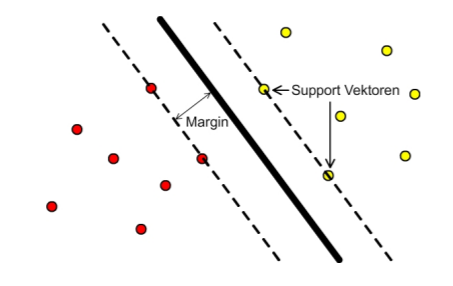
\includegraphics{abbildungen/sv.PNG}
	\caption{Die Abbildung zeigt die optimale trennende Hyperebene zwischen den gelben und roten Datenvektoren, sowie die jeweiligen Support-Vektoren.}
	\label{img:sv}
\end{figure}

Wir wollen abschließend die Überlegung aus \ref{bem-hard-svm} (b), sowie die Lösbarkeit und Äquivalenz der Probleme (\ref{svm-min-max-nb}), (\ref{svm-min-max}) und (\ref{hard-svm}) in einem Lemma festhalten.

\begin{lemma}
	\label{lemma-svm-prob-aequ}
	Die Probleme (\ref{svm-min-max-nb}), (\ref{svm-min-max}) sowie (\ref{hard-svm}) sind äquivalent und lösbar.
\end{lemma}
\begin{proof}
	Die Äquivalenz von den Problemen (\ref{svm-min-max}) und (\ref{hard-svm}) folgt (nach einer Normierung der Zielfunktion um den Faktor $2$) mit Lemma 15.2 in \cite{sb-umlfta}. Die Aussage folgt dann mit Lemma \ref{lemma-svm-minmax-equ} und Lemma \ref{lemma-hard-svm-loes}.
\end{proof}

\section{Homogene SVMs}
Die \emph{homogene SVM} überführt zunächst die separierbaren Datenvektoren $(x^1,y^1),...,(x^l,y^l)$ über die \emph{Einbettung}
$$
\widehat{(\, \cdot \, )} : \mathbb{R}^n \rightarrow \mathbb{R}^{n+1},\ \hat{x} := (x,1).
$$
in den $\mathbb{R}^{n+1}$. Die eingebetteten Datenvektoren kennzeichnen wir mit
$$
\hat{x}^1,...,\hat{x}^l \in \mathbb{R}^n \times \mathbb{R} = \mathbb{R}^{n+1}.
$$
Es ist ersichtlich, dass die eingebetteten Datenvektoren $\hat{x}^1,...,\hat{x}^l$ durch eine homogene Hyperebene $E_{(\tilde{w},0)} \subset \mathbb{R}^{n+1}$ separiert werden können. Analog zum Hard-SVM wählt die homogene SVM nun die homogene Ebene, die den Abstand zu den eingebetteten Datenvektoren maximiert. Dies führt uns wie im vorherigen Unterkapitel auf die

\begin{definition}[Homogene SVM]
Das durch 
\begin{equation}
\label{equ-homog-svm}
\begin{aligned}
	\min_{\tilde{w} \in \mathbb{R}^{n+1}} \; \frac{1}{2} ||\tilde{w}||^2 \qquad
	\text{u.d.N.} \qquad  
	y^i \langle \hat{x}^i, \tilde{w} \rangle \geq 1
\end{aligned}
\end{equation}
definierte Optimierungsproblem bezeichnen wir als homgene SVM.
\end{definition}

\begin{bemerkung}
\begin{itemize}
\item[(a)] Die Lösbarkeit von (\ref{equ-homog-svm}) kann analog zum Lemma \ref{lemma-hard-svm-loes} gezeigt werden. 
Fassen wir $\tilde{w}$ als $(w,b) \in \mathbb{R}^n \times \mathbb{R}$ auf, lässt sich die homogene SVM auch in der Form
$$
\begin{aligned}
\min_{(w,b)} \; \frac{1}{2} \left( ||w||^2 + b^2 \right) \qquad
\text{u.d.N.} \qquad  y^i (\langle x^i, w \rangle +b) \geq 1
\end{aligned}
$$
schreiben. Damit kann die homogene SVM als Hard-SVM aufgefasst werden, bei der zusätzlich der Term $b$ regularisiert wird.
\item[(b)] Wir werden im nächsten Unterkapitel sehen, dass bei der Dualisierung der homogenen SVM eine Nebenbedingung wegfällt. Dies wird uns später bei der Formulierung der Koordinatenabstiegsmethode sehr zu pass kommen.
\item[(c)] Das Beispiel \ref{bsp-homg-nequ-hard} zeigt, dass sich die Lösungen der Hard-SVM und der homogenen SVM im Allgemeinen unterscheiden. Nach \cite{sb-umlfta} ist dieser Unterschied für das Klassifizierungsproblem in der Praxis jedoch oft nicht spürbar.
\end{itemize}
\end{bemerkung}
 
\begin{beispiel}
\label{bsp-homg-nequ-hard}
Seien
$$
\begin{aligned}
	x^1 &= (1,\ 2)^t  &x^2  &= (1,\ 0)^t \\
	y^1 &= 1 		  &y^2 &= -1
\end{aligned}
$$
die Datenvektoren für die beiden Klassen $L=\{ y^1,\ y^2 \} = \{1,\ -1 \}$. Nach einer Modifikation für das homogene SVM erhalten wir 
die Datenvektoren
$$
\begin{aligned}
	\hat{x}^1 &= (1,\ 2,\ 1)^t &\hat{x}^2 &= (1,\ 0,\ 1)^t \\
	 y^1 &= 1					 &y^2 &= -1
\end{aligned}.
$$


\begin{figure}[htbp]
	\centering
	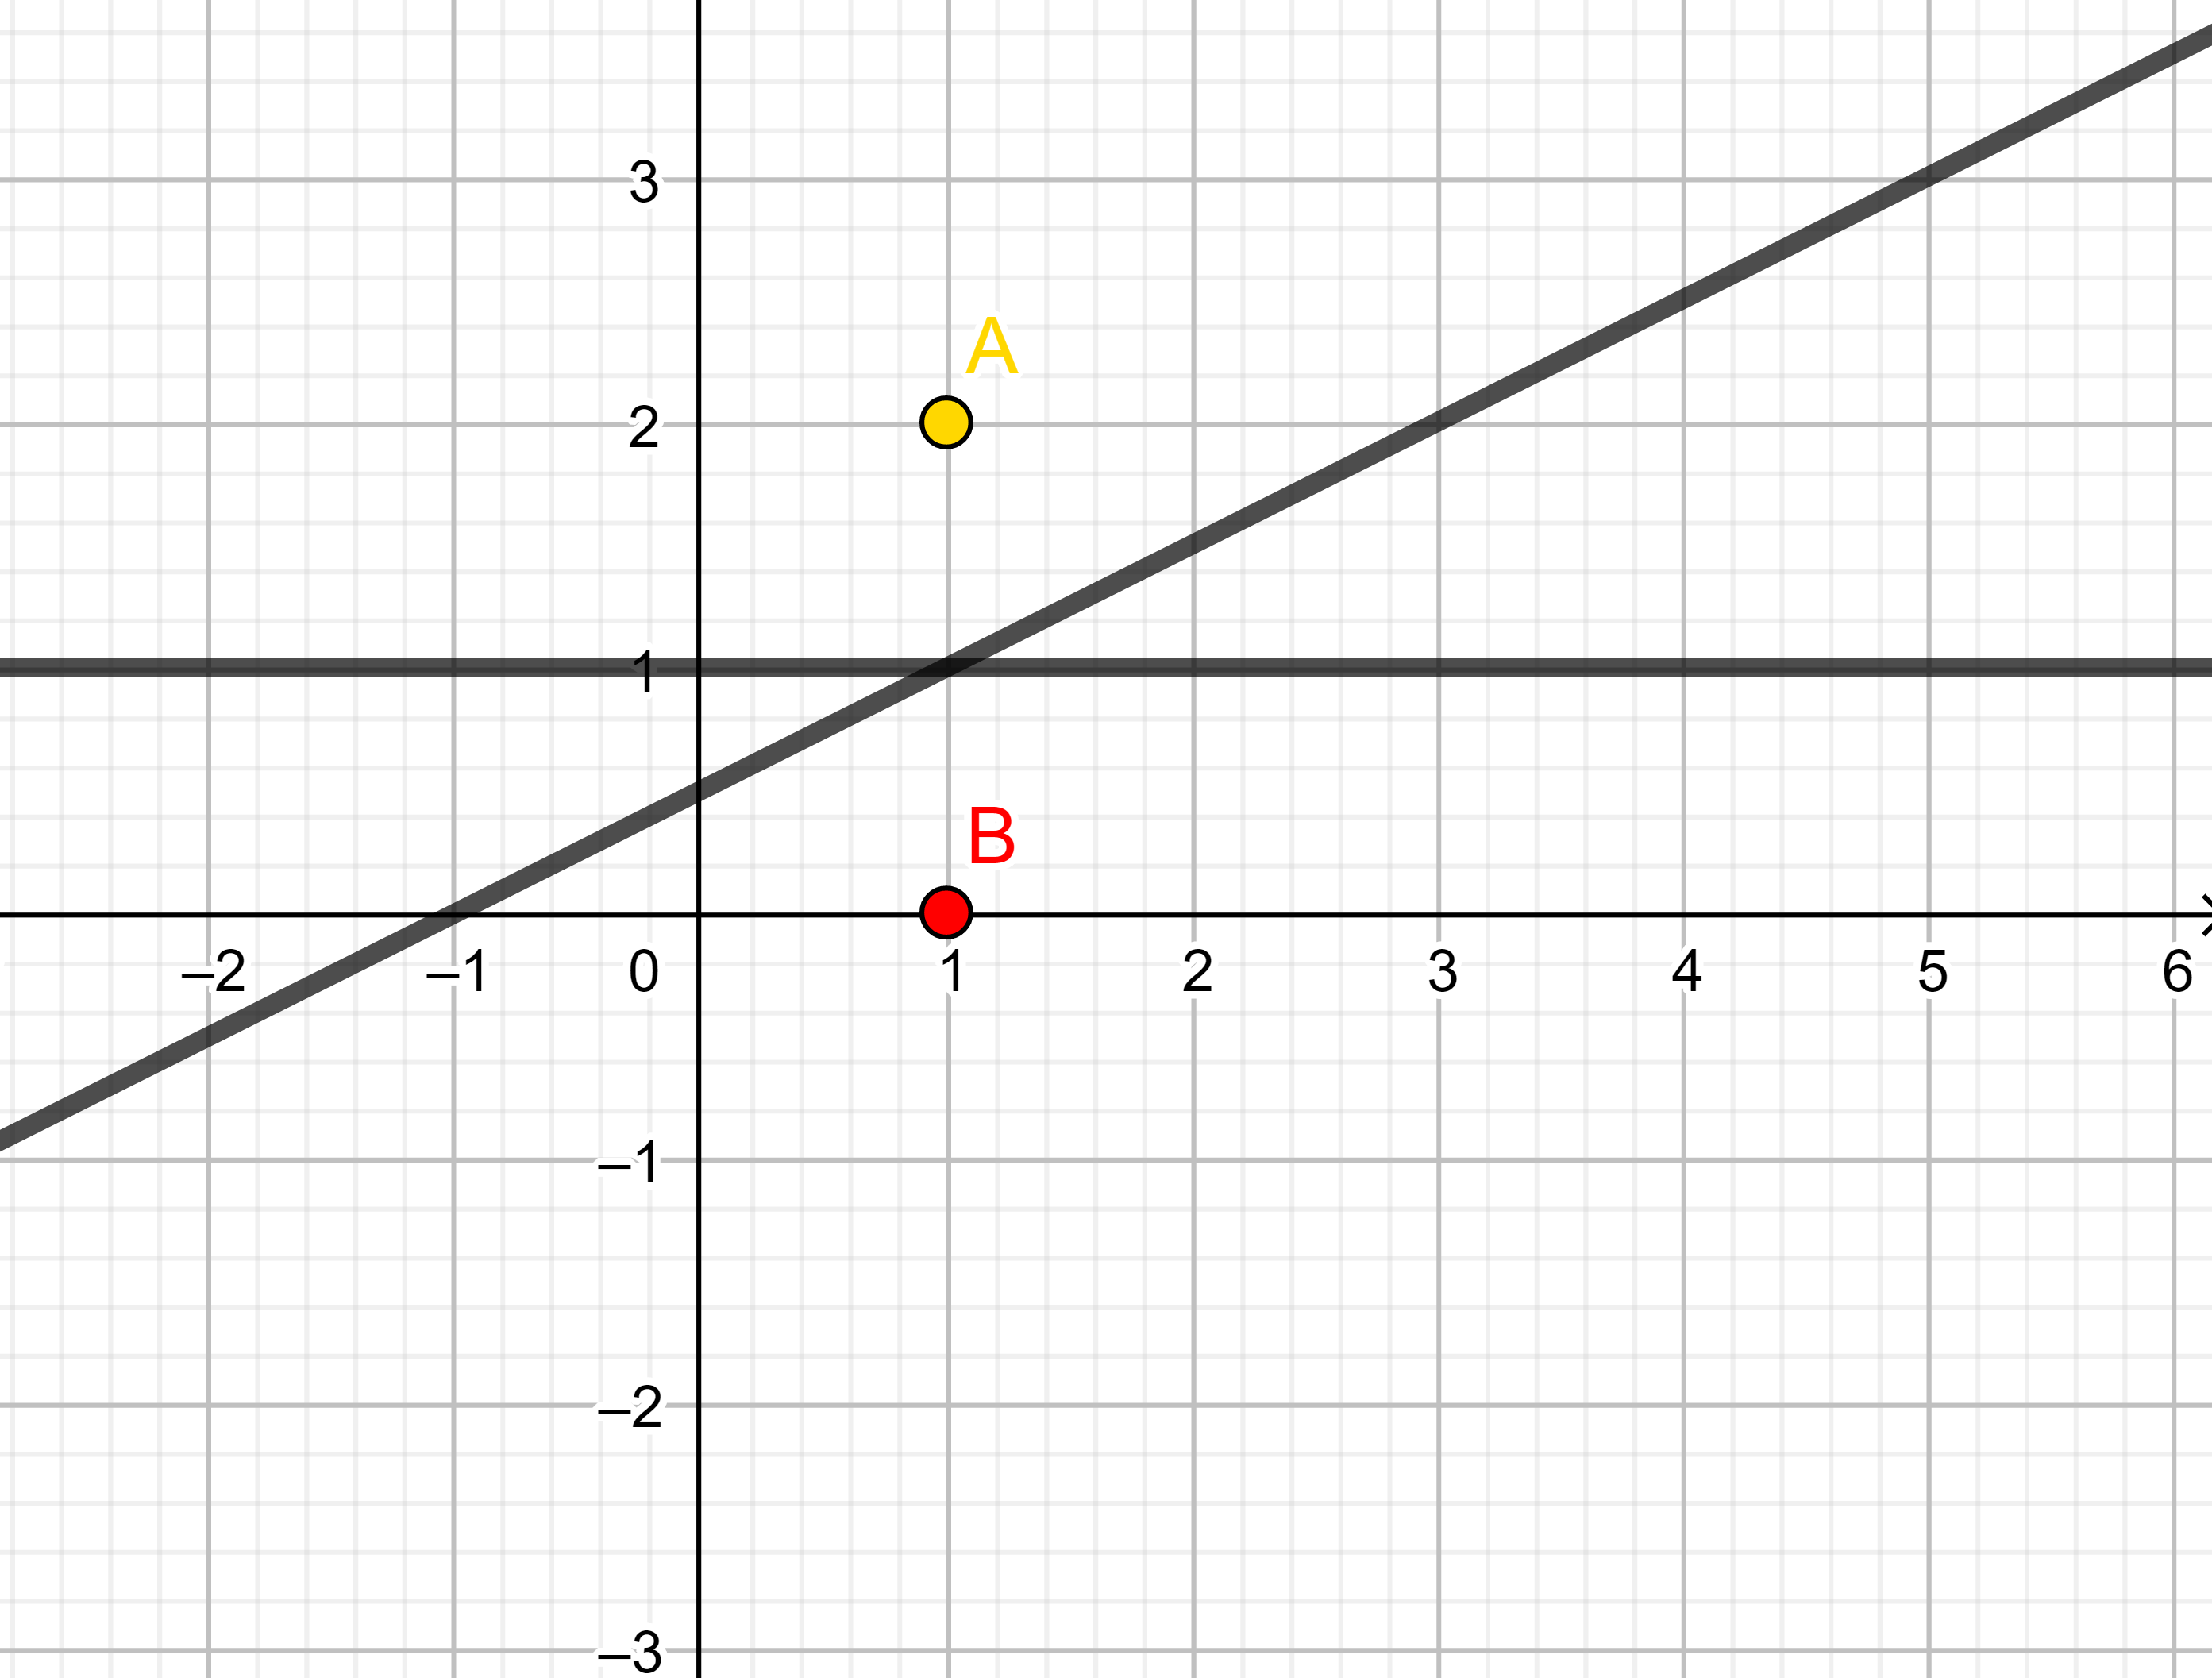
\includegraphics{abbildungen/homogen.png}
	\caption{Die Abbildung zeigt die Lösung vom Hard- bzw. homogenen SVM für die Datenvektoren $A=x^1 = (1, 2)^t$ und $B=x^2 = (1,0)^t$ im $\mathbb{R}^2$.}
	\label{img:hardvssoft}
\end{figure}

Für das Hard- bzw. homogene SVM ist eine Hyperebene $(w,b) \in \mathbb{R}^{2+1}$ bzw. $\tilde{w} := (w,b) \in \mathbb{R}^{3}$ gesucht, die den Restriktionen
$$
\begin{aligned}
	w_1 + 2w_2 + \, b -1 \geq 0 \\
	w_1 + \, b +1 \geq 0,
\end{aligned}
$$
beziehungsweise 
$$
\begin{aligned}
	0 &\geq -w_1 - 2w_2 - b + 1 \\
	0 &\geq  w_1 + b + 1
\end{aligned}
$$
genügt, wobei $w_i$ die i-te Komponente von $w$ bezeichnet. Während die Restriktionen bei der Hard- und homogenen SVM übereinstimmen, ändert sich bei der homogenen SVM die Zielfunktion von
$$
	\min_{(w,b)} \; \frac{1}{2} (w_1^2+w_2^2).
$$
zu
$$
	\min_{(w,b)} \; \frac{1}{2} (w_1^2+w_2^2+b^2).
$$
Wie auf der Abbildung \ref{img:hardvssoft} zu erkennen ist, ergibt sich die normierte Lösung der Hard-SVM durch die Hyperebene $\{ (x_1,x_2) \in \mathbb{R}^2 \ | \ x_2=1 \} \subset \mathbb{R}^2$. 
Um die Lösung der homogenen SVM zu ermitteln, suchen können wir das Gleichungssystem
$$
	\nabla \left( \frac{1}{2}(w_1^2+w_2^2+b^2) \right) = 
	\begin{pmatrix} w_1 \\ w_2 \\ b \end{pmatrix} = 
	\begin{pmatrix} 
		-\lambda_1 + \lambda_2 \\ -2 \lambda_1 \\ -\lambda_1 + \lambda_2 
	\end{pmatrix} = 
	- \lambda_1 \begin{pmatrix} 1 \\ 2 \\ 1 \end{pmatrix} +
	\lambda_2 \begin{pmatrix} 1 \\ 0 \\ 1 \end{pmatrix}
$$
lösen. Erhalten wir damit einen KKT-Punkt, müssen wir diesen Schritt nicht näher erläutern. Eingesetzt in die Restriktionen ergibt dies
$$
\begin{aligned}
	6 \lambda_1 & - 2 \lambda_2 \geq 1 \\
	-2 \lambda_1 &+ 2 \lambda_2 \geq 1,
\end{aligned}
$$
woraus $\lambda_1 \geq \frac{1}{2} ,\ \lambda_2 \geq 1$ folgt. Um einen KKT-Punkt zu erhalten setzen wir schließlich $\lambda_1 = \frac{1}{2} ,\ \lambda_2=1$. Damit ist $(w_1, w_2, b) = (\tfrac{1}{2}, -1, \tfrac{1}{2})$. Die Hyperebene im $\mathbb{R}^2$ ist also durch $ \{ (x_1,x_2) \in \mathbb{R}^2 \ | \ \tfrac{1}{2}x_1-x_2+\tfrac{1}{2} = 0  \} \subset \mathbb{R}^2$ gegeben.
\end{beispiel}


Um die Notationen zu vereinfachen werden wir im homogenen Fall immer annehmen, dass die Trainingsdaten a priori in den $\mathbb{R}^{n+1}$ eingebettet wurden. Wir können in diesem Fall also wieder davon ausgehen, dass $\hat{x}^i \in \mathbb{R}^n$ und schreiben $x^i$ statt $\hat{x}^i$, sowie $w$ statt $\tilde{w}$. Auch in den nächsten Abschnitten werden wir dies so fortführen.

\section{Soft-SVMs}
Wir wollen zunächst anmerken, dass wir für die \emph{Soft-SVM} wieder den homogenen Fall annehmen. \\

Die lineare Separierbarkeit (Definition \ref{def-lin-sep}) ist eine sehr harte Anforderung an die Datenvektoren $(x^1,y^1),...,(x^l,y^l)$ und in der Praxis nicht immer anzutreffen. Aus diesem Grund führen wir in der nächsten Definition ein neues Problem ein, das die Anforderung durch die \emph{Schlupfvariable} $\xi = (\xi_1 ,...,\xi_l) \in \mathbb{R}^l$ abschwächt.

\begin{figure}[h]
	\centering
	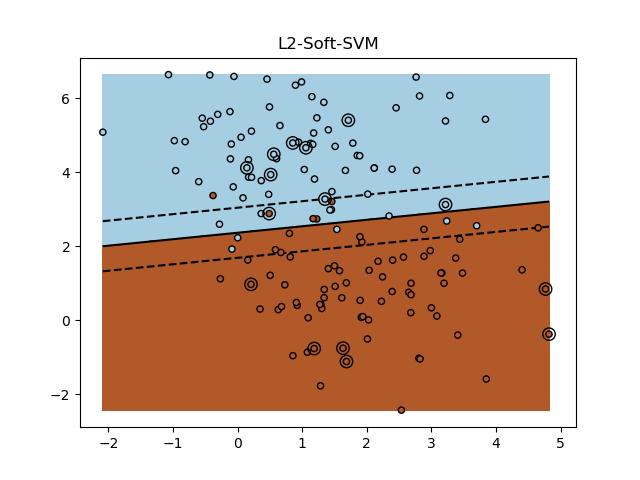
\includegraphics[scale=0.90]{abbildungen/softsvm_ex1.png}
	\caption{Illustrierung eines Klassifizierungsproblems. Die schwarze durchgezogene Linie zeigt die durch die L2-Soft-SVM ermittelte Hyperebene. Die gestrichelte Linie deutet den Margin an. (Die doppelt umrandeten Datenvektoren haben nicht zur Modellbildung beigetragen. Bei diesen Vektoren handelt es sich also um \emph{Testvektoren}.)}
	\label{img:softsvm}
\end{figure}

\begin{definition}[L1/L2-Soft-SVM]
	Seien $p=1,2,\ C > 0$. Dann ist die Lp-Soft-SVM definiert durch
	\begin{equation}
	\label{soft-svm-slack1}
	\begin{aligned}
		& \smash{ \argmin_{(w,\xi) \in \mathbb{R}^n \times \mathbb{R}^l}{
			\frac{1}{2}||w||^2+C\sum_{i=1}^{l}{\xi_i^p}
		}}
		\qquad \text{u.d.N.} \qquad
		& y^k \langle w, x^k \rangle &\geq 1 - \xi_k \\
		&& \xi_k &\geq 0 \\
		&& k &= 1,...,l.
	\end{aligned}
	\end{equation}
\end{definition}
Zu erkennen ist, dass der Schlupf $\xi$ die Lösbarkeit von $(\ref{soft-svm-slack1})$ sicherstellt; auch dann, wenn die Datenvektoren $(x^1,y^l),...,(x^l,y^l)$ nicht separierbar sind.

Definieren wir $$\ell_i^p(x,b) := \max(1-y^i\langle w, x^i \rangle,\ 0)^p,$$ für $i=1,...,l$, so stoßen wir auf die
\begin{definition}[SVM mit L1/L2 hinge loss]
	Seien $p=1,2,\ C > 0$. Dann ist die $L_p$-Soft-SVM mit \emph{hinge-loss} definiert durch
	\begin{equation}
	\label{soft-svm-loss1}
	\begin{aligned}
	\argmin_{w \in \mathbb{R}^n}{\frac{1}{2}||w||^2+C\sum_{1}^{l}{\ell_i^p(w)}}.
	\end{aligned}
	\end{equation}
\end{definition}

\begin{lemma}
	\label{lemma-soft-loesbar}
	Die Probleme (\ref{soft-svm-slack1}) und (\ref{soft-svm-loss1}) sind lösbar und äquivalent. 
\end{lemma}
\begin{proof}
	Ein Beweis wird in Behauptung 15.5 \cite{sb-umlfta} für den Fall $p=1$ geliefert: Fixiere $(w,b)$ und minimiere über $\xi$ bezüglich des Problems (\ref{soft-svm-slack1}). Wegen $\xi \geq 0$ ist $\xi_i = 0$, genau dann wenn $y^i(\langle w, x^i \rangle +b) \geq 1$ und $\xi_i = 1-y^i(\langle w, x^i \rangle +b)$ im anderen Fall. Da $(w,b)$ beliebig waren, gilt dies auch für das Minimum. Damit ist die Behauptung gezeigt. Den Fall $p=2$ zeigt man analog.
\end{proof}

\section{Duale SVM-Probleme}
Im Folgenden werden wir die \emph{dualen Probleme} der vorherigen \emph{primalen Probleme} herausarbeiten. Sie sind oft - auch in dieser Arbeit - Grundlage algorithmischer Lösungsverfahren. Zunächst zeigen wir jedoch ein vorbereitendes Hilfslemma.

\begin{lemma}
	Seien $\alpha \geq 0 \in \mathbb{R}^n$,
	\begin{equation}
	\begin{aligned}
	G_{\alpha}: \mathbb{R}^n \rightarrow \mathbb{R}, w \mapsto \frac{1}{2}||w||^2 + \sum_{i=1}^{l} \alpha_i (1- y^i( \langle w, x^i \rangle)), \\
	q(\alpha) := \sum_{i=1}^{l}\alpha_i - \frac{1}{2} \left< \sum_{j=1}^{l} \alpha_j y^j x^j ,\ \sum_{j=1}^{l} \alpha_j y^j x^j \right>.
	\end{aligned}
	\end{equation}Die Funktion $G_\alpha$ besitzt ihr Minimum bei $w^* = \sum_{1}^{l} \alpha_i y^i x^i$. Weiter ist $G_{\alpha}(w^*) = q(\alpha)$.
\end{lemma}
\begin{proof}
	Nach Satz \ref{satz-strict-konvex-innprdt} ist der erste Summand von $G_\alpha$ konvex. Da der zweite Summand als lineare Funktion konvex ist und Linearkombinationen konvexer Funktionen konvex sind, ist $G_\alpha$ konvex. Nach Satz \ref{dual-kkt} ist $G_{\alpha}(w)$  also genau dann minimal, wenn $(w)$ ein KKT-Punkt ist. Aus der ersten KKT-Bedingungen ergibt sich für das Minimum von $G_\alpha$ die Bedingung $\nabla G_\alpha(w) = w - \sum_{i=1}^{l} \alpha_i y^i x^i = 0 \Leftrightarrow w = \sum_{i=1}^{l} \alpha_i y^i x^i$. Die letzte Behauptung zeigt die Rechnung 
	$$
	\begin{aligned}
	G_\alpha(w^*) &= \left | \left |\sum_{1}^{l} \alpha_i y^i x^i \right | \right |^2 +
	\sum_{i=1}^l \alpha_i \left (1-y^i \left \langle \sum_{1}^{l} \alpha_i y^i x^i, x^i \right \rangle \right ) = \\
	&=\sum_{i=1}^{l}\alpha_i - \frac{1}{2} \left< \sum_{j=1}^{l} \alpha_j y^j x^j ,\ \sum_{j=1}^{l} \alpha_j y^j x^j \right> = q(\alpha).
	\end{aligned}
	$$
\end{proof}

Für den nächsten Satz merken wir noch an, dass die primalen Probleme aus konvexen und stetig differenzierbaren Zielfunktionen sowie affin linearen Nebenbedingungen bestehen, sodass die im Anhang vorgestellte Dualitätstheorie für restringierte Optimierungsprobleme in ihrer Gänze anwendbar ist.

\begin{satz}[Die dualen SVM-Probleme]
	\label{satz-svm-dual-probleme}
	Sein $q$ und $G_\alpha$ wie im vorherigen Lemma definiert. Es gelten die Aussagen:
\begin{itemize}
	\item[(i)] Das duale Problem der Hard-SVM lautet $\max_{\alpha \geq 0} q(\alpha)$ u.d.N. $\sum_{i=1}^l \alpha_i y^i = 0$.
	\item[(ii)] Das duale Problem der homogenen SVM lautet $\max_{\alpha \geq 0} q(\alpha)$.
	\item[(iii)] Das duale Problem der L1-Soft-SVM lautet $\max_{C \geq \alpha \geq 0} q(\alpha)$
	\item[(iv)] Das duale Problem der L2-Soft-SVM mit lautet $\max_{\alpha \geq 0} q(\alpha)-\frac{1}{4C}\sum_{i=1}^{l} \alpha_i^2$.
\end{itemize}
\end{satz}
\begin{proof}
Zu (i): Die \emph{Lagrange-Funktion} für die Hard-SVM ist
$$
L(w,b,\alpha) = \frac{1}{2}||w||^2 + \sum_{i=1}^{l}\alpha_i(1-y^i(
\langle w,x^i \rangle) + b) = G_{\alpha}(w) - \sum_{i=1}^{l}\alpha_i y^i b.
$$
Für $\sum_{i=1}^{l}y^i \alpha_i \neq 0$ ist $\inf_{(w,b)} L(w,b,\alpha) = -\infty$, weshalb wir uns für das duale Problem auf $\sum_{i=1}^{l}y^i \alpha_i = 0$ beschränken können. Das duale Problem der Hard-SVM ist damit gegeben durch
$$
\begin{aligned}
\max_{\alpha \geq 0} \inf_{(w,b)} L(w,b,\alpha) = 
\max_{\alpha \geq 0} \min_w G_{\alpha}(w) = \max_{\alpha \geq 0}q(\alpha) \\
\text{u.d.N} \; \sum_{i=1}^l \alpha_i y^i = 0.
\end{aligned}
$$.

Zu (ii): Die Lagrange-Funktion für die homogene SVM ist
$$
L(w,\alpha) = \frac{1}{2}||w||^2 + \sum_{i=1}^{l}\alpha_i(1-y^i 
\langle w,x^i \rangle) = G_{\alpha}(w).
$$
Das duale Problem der homogenen SVM ist damit gegeben durch
$$
\max_{\alpha \geq 0} \inf_{(w,b)} L(w,b,\alpha) = 
\max_{\alpha \geq 0} \min_w G_{\alpha}(w) = \max_{\alpha \geq 0}q(\alpha)
$$.


Zu (iii): Die Lagrange-Funktion vom Problem \ref{soft-svm-slack1} ist gegeben durch 
$$
\label{lagrange-l1-softsvm1}
\begin{aligned}
L(w, \xi, \alpha, \beta) &:= \tfrac{1}{2}||w||^2 + C \sum_{i=1}^l \xi_i 
+ \sum_{i=1}^{l}{\alpha_i (1-y^i w^t x^i - \xi_i)} - \sum_{i=1}^{l} \beta_i \xi_i = \\
&= \tfrac{1}{2} ||w||^2 + \sum_{i=1}^{l}{\alpha_i (1-y^i w^t x^i)} + \sum_{i=1}^{l}(C-\alpha_i - \beta_i)\xi_i \\
&= G_{\alpha}(w) + \sum_{i=1}^{l}(C-\alpha_i - \beta_i)\xi_i.
\end{aligned}
$$
Für $C \neq \alpha_i + \beta_i$ für ein $i \in \{1, ..., l\}$ ist $\inf_{w,\xi}L(w,\xi,\alpha,\beta) = -\infty$. Wir dürfen also für das duale Problem $C_i = \alpha_i+\beta_i$ für alle $i = 1,...,l$ annehmen. Also muss die Bedingung $0 \leq \alpha \leq C$ gelten. Das duale Problem der L1-Soft-SVM ist damit gegeben durch
$$
\max_{C \geq \alpha \geq 0} \inf_{(w,b)} L(w,b,\alpha) = 
\max_{C \geq \alpha \geq 0} \min_w G_{\alpha}(w) = \max_{C \geq \alpha \geq 0}q(\alpha).
$$

Zu (iv): Die Lagrange-Funktion ist damit gegeben durch
$$
\begin{aligned}
L(w,\xi,\alpha,\beta) &= \frac{1}{2}||w||^2+\sum_{i=1}^l \alpha_i(1-y^i \langle w, x^i \rangle ) + \sum_{i= 1}^l \left(C \xi_i^2 - \alpha_i \xi_i - \beta_i \xi_i \right) \\
&= G_\alpha(w) + \sum_{i= 1}^l \left(C \xi_i^2 - \alpha_i \xi_i - \beta_i \xi_i \right).
\end{aligned}
$$
Der von $\xi$ abhängige Term ist nach Satz \ref{dual-kkt} minimal bei $\xi = \tfrac{1}{2}(\alpha + \beta)$. Nach Satz \ref{dual-satz} ist die duale Lösung gepaart mit einer primalen Lösung ein KKT-Punkt. Für eine mögliche Lösung muss also wegen des Komplementären Schlupfs $\beta^t \xi = 0$ gelten. Wegen $\beta \geq 0, \alpha \geq 0$ erhalten wir insgesamt, dass für eine duale Lösung $\beta  = 0$ gelten muss. Das duale Problem der L2-Soft-SVM ist damit gegeben durch
$$
\begin{aligned}
\max_{\alpha \geq 0, \beta \geq 0} \inf_{w,\xi \geq 0} L(w,\xi,\alpha,\beta) =
\max_{\alpha \geq 0} 
q(\alpha) + \sum_{i= 1}^l C(\tfrac{1}{2C}\alpha)^2 - \tfrac{1}{2C} \alpha^2 = 
\max_{\alpha \geq 0} q(\alpha) - \sum_{i= 1}^l \tfrac{1}{4C}a_i^2.
\end{aligned}
$$
\end{proof}

\begin{bemerkung}\label{bem:duale-probleme}
\begin{itemize}
\item[(a)] Die Lösbarkeit der dualen Probleme aus dem vorherigen Satz sieht man mit Hilfe von Satz \ref{dual-kkt}, Satz \ref{dual-satz} und der bereits gezeigten Lösbarkeit der jeweiligen primalen Probleme.
\item[(b)]
Für den Fall (i) aus dem vorherigen Satz zeigen wir exemplarisch, wie wir aus der dualen Lösung $\alpha^*$ die primale Lösung $(w^*,b^*)$ erhalten. Wegen  Satz \ref{dual-satz} ist $(w^*,b^*,\alpha^*)$ ein KKT-Punkt. Aus den KKT-Bedingungen folgt, dass 
$$
\nabla_w L(w^*,b^*,\alpha^*) = 0 \Leftrightarrow \nabla G_{\alpha^*}(w^*) = 0 \Leftrightarrow w^* = \sum_{i=1}^{l}y^i \alpha_i^* x^i.
$$ 
Um $b^*$ zu ermitteln, sei hierzu ein $i \in \{1, ..., l\}$ mit $\alpha_i^* > 0$. Wegen des komplementären Schlupfs gilt dann 
$$
1-y^i(\langle w^*, x^i \rangle) + b^* = 0 \Leftrightarrow b^* = -1+y^i(\langle w^*, x^i \rangle).
$$
\item[(c)]
\label{svm-eindeutigkeit}
Für die Fälle (ii) bis (iv) gilt mit analoger Begründung die Beziehung 
$w^* = \sum_{i=1}^{l}y^i \alpha_i^* x^i$ wobei $w^*$ und $\alpha^*$ die jeweiligen Teillösungen der primalen bzw. dualen Probleme sind. 
Weiter folgt aus den Fällen (iii) und (iv), dass mit $\xi^* = \ell^1(w^*):=(\ell_1^1(w^*),...,\ell_l^1(w^*))$ der Vektor $(w^*,\xi^*)$ eine Lösung für das jeweilige primale Problem ist.

\item [(d)] Aus (b) und (c) folgen, dass die primale Lösung für die Probleme (i) bis (iv) eindeutig bestimmt sind.

\item[(e)] Führt man für die Hard-SVM analog zur Soft-SVM Schlupfvariablen ein, ist die primale Lösung im Allgemeinen nicht eindeutig bestimmt, wie in \cite{bcc-unqu-2000} gezeigt wird.
\end{itemize}
\end{bemerkung}

\begin{korollar}
	\label{korollar-prim-uniqu}
	Die Probleme (\ref{hard-svm}), (\ref{svm-min-max-nb}) und (\ref{svm-min-max}) sind eindeutig lösbar.
\end{korollar}
\begin{proof}
	Die Behauptung folgt mit Lemma \ref{lemma-hard-svm-loes}, Lemma \ref{lemma-svm-prob-aequ} und Bemerkung \ref{svm-eindeutigkeit} (c).
\end{proof}

Wie wir sehen, handelt es sich bei den dualen Problemen um restringierte Optimierungsprobleme im $\mathbb{R}^l$, bei den primalen um Optimierungsprobleme im $\mathbb{R}^n$.


\chapter{Abstiegsverfahren}
Wir wollen in diesem Abschnitt ein hinreichendes Konvergenzkriterium herleiten. Hierfür führen folgende Notationen und Definitionen ein:
\begin{itemize}
\item Seien $X$, $\mathcal{Z} \subset X$ Mengen.
\item Sei $\Phi : X \rightarrow \mathbb{R}$ so, dass das Problem 
$
	\min_{z \in \mathcal{Z}} \Phi(z)
$
lösbar ist. Weiter setzen wir $c^* := \min_{z \in \mathcal{Z}} \Phi(z)$, sowie $\mathcal{Z^*} := \Phi^{-1}(c^*)$.

\item Sei $\mathcal{F} : Z \rightarrow Z$ so, dass $\Phi(\mathcal{F}(x)) < \Phi(x)$ für alle $x \in \mathcal{Z} \setminus \mathcal{Z^*}$ und $\Phi(\mathcal{F}(x)) = \Phi(x)$ für alle $x \in \mathcal{Z}^*$. Wir nennen $\mathcal{F}$ Abstiegsfunktion, oder einfach Abstieg für $\mathcal{Z}$ und bezeichnen $\mathcal{F}(z)$ Abstieg an $z$ auf $\Phi$ über $\mathcal{F}$. Weiter setzen wir $\mathcal{F}^i := 
\underbrace{\mathcal{F} \circ ... \circ \mathcal{F}}_{i \; \text{mal}}$, sowie $\mathcal{F}^* \Phi(x) := \lim_{i \rightarrow \infty}\Phi^(\mathcal{F}^i(x))$.

\item Sei $N(\varepsilon, c) := \Phi^{-1}([ \; c^* + \varepsilon,\ c \; ]) \; \cap \; \mathcal{Z}$ beziehungsweise
$
N(\varepsilon) := N(\varepsilon, \infty) := 
\bigcup\limits_{c \geq c^*+\varepsilon} N(\varepsilon,c) $  
die $c$-Sublevelmenge zum Niveau $\varepsilon$.

\item Sei 
$
M(\varepsilon,c) := 
\sup_{x \in N(\varepsilon,c)} \; \frac{\Phi(\mathcal{F}(x)) - c^*}{\Phi(x)-c^*}
$
beziehungsweise $M(\varepsilon) := M(\varepsilon, \infty)$
der minimale Relativabstieg auf $N(\varepsilon,c)$ über $\mathcal{F}$.

\item Das Quadrupel $(X ,\ \mathcal{Z} ,\ \Phi ,\ \mathcal{F})$ bezeichnen wir als Abstiegsverfahren.


\end{itemize}

\begin{bemerkung}
\begin{itemize}
\item[(a)] Für alle $\varepsilon > 0, \ c > c^* + \varepsilon$ beziehungsweise $c = \infty$ ist $M(\varepsilon, c)$ wohldefiniert und es gilt $0 \leq M \leq 1$.
\item[(b)] $\mathcal{F}^* \Phi$ ist wohldefiniert und auf $\mathcal{Z}$ gilt $c^* \leq \mathcal{F}^* \Phi \leq \Phi$.
\end{itemize}	
\end{bemerkung}

\begin{satz}
	Sei $(X ,\mathcal{Z}, \Phi , \mathcal{F})$ ein Abstiegsverfahren. Sei weiter $M(\varepsilon) < 1$ für beliebiges $\varepsilon > 0$. Dann ist $\mathcal{F}^* \Phi = c^*$.
\end{satz}
\begin{proof}
	Sei $x \in \mathcal{Z}^*$. Nach Definition von  von $\mathcal{F}$ ist dann $\mathcal{F}(x) = x$. Also ist $\mathcal{F}^* \Phi(x) = x$. 
	
	Sei nun $\varepsilon > 0$ und $x \in \mathcal{Z} \setminus \mathcal{Z}^*$. Sei weiter $x \in N(\varepsilon)$.
	Dann ist nach Definition von $M(\varepsilon)$
	$$
	\frac{\Phi(\mathcal{F}(x)) - c^*}{\Phi(x) - c^*} \leq M(\varepsilon) \Leftrightarrow
	\Phi(\mathcal{F}(x)) - c^* \leq M(\Phi(x) - c^*).
	$$
	Für $i \geq 1$ und $\mathcal{F}^i(x) \in N(\varepsilon)$ folgt induktiv, dass
	$$
	\Phi(\mathcal{F}^i(x)) - c^* \leq M^i (\Phi(x) - c^*).
	$$
	Da nach Voraussetzung $M(\varepsilon) < 1$, muss nach Definition von $N(\varepsilon)$ ein $j \in \mathbb{N}$ existieren, dass $\mathcal{F}^j(x) \in \mathcal{Z} \setminus N(\varepsilon)$.
	
	Sei nun $j \geq 0$ so, dass $\mathcal{F}^j(x) \in \mathcal{Z} \setminus N(\varepsilon)$. Dann ist nach Definition von $N(\varepsilon)$, $\mathcal{F}$ und Bemerkung 2.1 (b)  $c^* \leq \mathcal{F}^* \Phi(x) \leq \Phi(\mathcal{F}^j(x)) \le c^* + \varepsilon$. 
	
	Da $\varepsilon$ und $x$ beliebig waren, folgt schließlich $\mathcal{F}^*\Phi = c^*$.
\end{proof}

\begin{korollar}
	\label{satz-abstiegsverfahren-konv}
	Seien $(X, \mathcal{Z}, \Phi, \mathcal{F})$ ein Abstiegsverfahren, $(X,d)$ ein metrischer Raum, sowie $(Z,d)$ ein durch selbigem $d$ induzierter metrischer Raum. Seien $\Phi$ und $\Phi \circ \mathcal{F}$ stetig (bezüglich $d$). Weiter sei für jedes $\varepsilon > 0$ sowie jedes $z \in \mathcal{Z}$ die Menge $N(\varepsilon, \Phi(z))$ (bezüglich $d$) kompakt. Dann ist $\mathcal{F}^* \Phi = c^*$. Ist zusätzlich das Minimum eindeutig durch $z^*$ bestimmt und $Z$ abgeschlossen, so ist $\lim_{i \rightarrow \infty} \mathcal{F}^i(z) = z^*$ für alle $z \in \mathcal{Z}$.
\end{korollar}
\begin{proof}
	Seien $\varepsilon > 0,\ z \in \mathcal{Z}$ beliebig. Die Funktion 
	$$	
	\frac{\Phi(\mathcal{F}(x)) - c^*}{\Phi(x) - c^*}
	$$ ist stetig und nimmt wegen der Kompaktheit von $N(\varepsilon, \Phi(z))$ nach dem Satz vom Minimum und Maximum (vgl. \cite{ae-ana1}) ihr Maximum an. Daher ist
	$$
	M(\varepsilon, \Phi(z)) := 
	\sup_{z \in N(\varepsilon, \Phi(z))} \frac{\Phi(\mathcal{F}(x)) - c^*}{\Phi(x) - c^*} = 
	\max_{z \in N(\varepsilon, \Phi(z))} \frac{\Phi(\mathcal{F}(x)) - c^*}{\Phi(x) - c^*}
	< 1.
	$$
	Nach dem vorherigen Satz [angewendet auf 
	$(X, \{ \Phi \leq \Phi(z) \}, \Phi, \mathcal{F})$] 
	ist $\mathcal{F}^* \Phi = c^*$ auf $\{ \Phi \leq \Phi(z) \}$. Insbesondere ist $\Phi(z) = c^*$. 
	
	Sei nun das Minimum eindeutig durch $z^*$ bestimmt und $\mathcal{Z}$ abgeschlossen, $U_{z^*}$ eine beliebige offene Umgebung um $z^*$. Dann ist $N := N(\varepsilon, c) \setminus U_{z^*}$ abgeschlossen. Da $z^*$ das einzige Minimum ist, muss $\inf \Phi(N) = \min \Phi(N) > c^*$ gelten. Also ist $\mathcal{F}^i(z) \in U_{z^*}$ für fast alle $i \in \mathbb{N}$. Da $U_{z^*}$ eine beliebige Umgebung war, folgt schließlich $\lim_{i \rightarrow \infty} \mathcal{F}^i(z) = z^*$.
\end{proof}


\chapter{Implementierung der L1/L2-Soft-SVM}
Wir werden in diesem Unterkapitel die Koordinatenabstiegsmethode für die duale $L_1/L_2$-Soft-SVM formulieren und ihre Konvergenz theoretisch begründen. Zunächst wollen wir die in Satz \ref{satz-svm-dual-probleme} formulierten Probleme 
$$\max_{C \geq \alpha \geq 0} q(\alpha) \qquad
	\text{beziehungsweise} \qquad 
	\max_{\alpha \geq 0} q(\alpha) - \frac{1}{4C}\sum_{i=1}^{l}\alpha_i^2
$$
in eine für uns geeignetere Form bringen. Zunächst bemerken wir, dass 
$$
\begin{aligned}
	q(\alpha) &= \sum_{i=1}^{l} \alpha_i - \frac{1}{2} \left< \sum_{i=1}^{l} \alpha_i y^i x^i ,\sum_{j=1}^{l} \alpha_j y^j x^j \right> =  
	\sum_{i=1}^{l} \alpha_i - \frac{1}{2} \sum_{i,j=1}^{l} \alpha_i \alpha_j y^i y^j \left< x^i, x^j \right> = \\
	&= \sum_{i=1}^{l} \alpha_i - \frac{1}{2} \alpha^t Q \alpha
\end{aligned}
$$
mit der positiv semidefiniten Matrix $Q_{ij} = y^i y^j \left<x^i, x^j \right> \in \mathbb{R}^{l \times l}$ gilt. \\


Um Notationen zu sparen werden wir $U \in \mathbb{R}$ und die Diagonalmatrix $D \in \mathbb{R}^{l \times l}$ für die $L_1$- respektive $L_2$-Soft-SVM fallweise definieren: Im Falle des L1-Soft-SVM setzen wir $U=C$ und $D_{ii} = 0$ für $i=1,...,l$. Im Falle des L2-Soft-SVM setzen wir  $U=\infty$ und $D_{ii} = 1/(2C)$ für alle $i=1,...,l$. Die Aussagen, die mit $U$ und $D$ formuliert werden (oder aus solchen Aussagen folgen), sind dann jeweils im Kontext des L1- respektive L2-SVM-Soft-SVMs zweimal zu lesen. In dieser Notation lässt sich das zum dualen L1- und L2-Soft-SVM-Problem äquivalente Problem dann zu
\begin{equation}\label{equ:op-impl}
	\min_{U \geq \alpha \geq 0} f(\alpha) := \min_{U \geq \alpha \geq 0} \frac{1}{2}\alpha^t \bar{Q} \alpha - \sum_{i=1}^{l} \alpha_i
\end{equation}
formulieren, wobei wir $\bar{Q} = Q+D$ setzen. \\

Wir wollen nun Problem (\ref{equ:op-impl}) mit der \emph{Koordinatenabstiegsmethode} lösen. Hierfür minimieren wir  für einen beliebigen zulässigen Startwert $\alpha$ die Zielfunktion $f$ \emph{komponentenweise} solange, bis $\alpha$ optimal ist. Dies führt uns auf das zu lösende Subproblem 
\begin{equation}\label{equ:dec-schritt}
 	\argmin_{d \in \mathbb{R}}f(\alpha+de_i) \qquad \text{u.d.N.} \qquad 0 \leq \alpha_i+te_i \leq U_p.
\end{equation}
für $i=1,...,l$. Die Zielfunktion kann zu  
$$
f(\alpha+de_i) =  \frac{1}{2}\bar{Q}_{ii}d^2 + r d + s
$$
für eindeutig bestimmte $r,s \in \mathbb{R}$ umformuliert werden. Bei (\ref{equ:op-impl}) handelt es sich also um ein restringiertes quadratisches Optimierungsproblem im $\mathbb{R}^1$. Wegen $Q_{ii} = y^i y^i \left<x^i, x^i \right> = \left< x^i, x^i \right>$ und der Voraussetzung $x^i \neq 0$ ist $\bar{Q}_{ii} > 0$. Damit ist das Problem (\ref{equ:op-impl}) sowohl für den L1- als auch den L2-Soft-SVM eindeutig lösbar. Weiter ist es ersichtlich, dass wir die globale Lösung ohne Nebenbedingungen orthogonal auf $[0, U]$ projizieren können, um das eindeutige Minimum im restringierten Fall zu bestimmen. Wir wollen deshalb zunächst die Lösung im unrestringierten Fall ermitteln. Dies führt uns auf die Gleichung
$$
\frac{d}{dt}f(\alpha+te_i) = 0 \Leftrightarrow \nabla f(\alpha+t e_i)^t e_i = [\bar{Q}(\alpha + te_i)]_i - 1 = \nabla f(\alpha)^t e_i + \hat{Q}_{ii}t \stackrel{!}{=}0.
$$
Damit ergibt sich der Koordinatenabstieg in der $i$-ten Komponente zu 
\begin{equation}
\label{equ:cd-step}
k^i(\alpha) :=
\min \left( \max \left( \alpha_i-\frac{\nabla_i f(\alpha)}{\bar{Q}_{ii}},\ 0 \right),\ U \right).
\end{equation}
Weiter definieren wir $\mathcal{K}^i := (\mathcal{K}^i_1,...,\mathcal{K}^i_l)$ durch
\begin{equation} 
\mathcal{K}^i_j(\alpha) := \left\{ \begin{array}{ll}
	\alpha_i 	&,\ i \neq j \\
	k^i (\alpha) &,\ \text{sonst}
\end{array} \right.
\end{equation}
sowie $\mathcal{F}' = \mathcal{K}^l \circ \cdots \circ \mathcal{K}^1$. In Algorithmus \ref{alg:cod-alg} wird die Koordinatenabstiegsmethode formal formuliert.

\begin{algorithm}
\KwIn{$\alpha$}
\KwOut{$\alpha$}
\While{$\alpha$ nicht optimal}{
	$\alpha \gets \mathcal{F}'(\alpha)$	
}
\caption{Koordinatenabstiegsmethode}
\label{alg:cod-alg}
\end{algorithm}

Im nächsten Unterkapitel werden wir ein Optimalitätskriterium für Algorithmus \ref{alg:cod-alg} herleiten. Weiter klären wir, dass wir aus dem \emph{dualen} $\alpha$ ein \emph{primales} $w$ erhalten können, dass bei Anwendung des Algorithmus gegen die primale (Teil-)Lösung vom L1/L2-Soft-SVM konvergiert.

\section{Konvergenz und Abbruchkriterium}

\begin{bemerkung}\label{bem:impl-abstieg}
	Setzen wir $G = [0,U]^l$, so ist $\mathcal{F}':G \rightarrow G$ offenbar eine stetige Selbstabbildung, und es gilt $f(\mathcal{F}'(\alpha)) \leq f(\alpha)$.
\end{bemerkung}

\begin{lemma}\label{lem:impl-abstieg}
	Sei $\alpha \in \mathbb{R}^l$ zulässig für das Optimierungsproblem (\ref{equ:op-impl}). Gilt $\mathcal{F}'(\alpha) = \alpha$, so ist $\alpha$ eine Lösung für (\ref{equ:op-impl}).
\end{lemma}
\begin{proof}
Es seien die Voraussetzungen für den Satz erfüllt. Sei also $\alpha \in \mathbb{R}^l$ und es gelte $\mathcal{F}'(\alpha) = \alpha$.  Dann ist 
$$
\begin{aligned}
\mathcal{F}'(\alpha) = \alpha & \Leftrightarrow (k^1(\alpha),...,k^l(\alpha)) = \alpha \\
& \Leftrightarrow \alpha_i = k^i(\alpha) \qquad \text{für alle} \ i = 1,...,l.
\end{aligned}
$$ 
Hieraus folgt, dass $\nabla_i f(\alpha) = 0$ für $0 < \alpha_i < U$, sowie $\nabla_i f(\alpha) \geq 0$ für $\alpha_i = 0$. Im Fall der L1-Soft-SVM folgt außerdem, dass $\nabla_i f(\alpha) \leq 0$ für $\alpha = U$ ist. Wir können mit $\alpha$ also einen KKT-Punkt konstruieren, der die KKT-Bedingungen erfüllt (vgl. Definition \ref{def:kkt}). Damit ist nach Satz \ref{dual-kkt} $\alpha$ eine Lösung für (\ref{equ:op-impl}).
\end{proof}

\begin{lemma}\label{lem:abstg-impl}
	Das Quadrupel $(\mathbb{R}^l, G, f, \mathcal{F}')$ ist ein Abstiegsverfahren.
\end{lemma}
\begin{proof}
Zunächst identifizieren wir $\mathbb{R}^l$ mit $X$, sowie $\mathcal{Z}$ mit $G=[0,U]^l$.
Wegen Bemerkung	\ref{bem:duale-probleme} (a) ist das Problem (\ref{equ:op-impl}) lösbar. Wir können also $f$ mit $\Phi$ identifizieren. Wegen Bemerkung \ref{bem:impl-abstieg} und Lemma $\ref{lem:impl-abstieg}$ können wir weiter $\mathcal{F}'$ mit $\mathcal{F}$ identifizieren. Damit ist $(\mathbb{R}^l, G, f, \mathcal{F}')$ ein Abstiegsverfahren.
\end{proof}

Sei $\alpha^0$ zulässig für (\ref{equ:op-impl}). Für $k > 1$ setzen wir $\alpha^k := (\mathcal{F}')^k(\alpha^0)$. 

\begin{satz}\label{satz:impl-grenz-opt}
	Sei $\alpha^*$ eine Lösung für (\ref{equ:op-impl}), dann gilt $\lim_{k \rightarrow \infty} f(\alpha^k) = f(\alpha^*)$.
\end{satz}
\begin{proof}
	Sei $c^* = f(\alpha^*)$ und $G$ die zulässige Menge das Problem (\ref{equ:op-impl}). 
	Wir müssen zeigen, dass $N' := N(\varepsilon,f(\alpha)) := f^{-1}([c^*+\varepsilon, f(\alpha)]) \cap G$ für ein beliebig zulässiges $\alpha \in G$ kompakt ist. Dann folgt die Aussage mit Lemma \ref{lem:abstg-impl}, Bemerkung \ref{bem:impl-abstieg} und Satz \ref{satz-abstiegsverfahren-konv}. \\ 
	
	Zunächst ist nach Theorem 2.20 in \cite{ae-ana1} $N'$ als Urbild einer abgeschlossener Menge unter einer stetigen Funktion abgeschlossen. 
	Für den L1-Soft-SVM folgt die Beschränktheit von $N'$ aus $N' \subset G = [0,C]^l$. Für den L2-Soft-SVM folgt die Beschränktheit von $N'$ aus der (echt) positiven Definitheit von $\hat{Q} = Q + CI$, mit der positiv semidefiniten Matrix $Q$ und der Einheitsmatrix $I \in \mathbb{R}^{l \times l}$. Damit ist nach dem Satz von Heine-Borel (vgl. \cite{ae-ana1}) $N'$ kompakt.
\end{proof}


\begin{definition} 
Die durch 
$$
\nabla_i^P f(\alpha) = \left\{ 
\begin{array}{ll}
	\nabla_i f(\alpha)  		 &,\ 0 < \alpha_i < U \\
	\min(0, \nabla_i f(\alpha))	 &,\ \alpha_i = 0 \\
	\max(0, \nabla_i f(\alpha))  &,\ \alpha_i = U
\end{array}
\right.
$$
definierte Abbildung bezeichnen wir als \emph{projizierten Gradienten}. Weiter setzen wir  
$$ 
	w(\alpha) := \sum_{i=1}^{l} \alpha_i y^i x^i.
$$.
\end{definition}

\begin{lemma}
Sei $\alpha \in \mathcal{Z}$ und sei $1 \leq i \leq l$. Sei weiter $(w^*, \xi^*)$ die primale Lösung der $L_1$-Soft-SVM. Dann gilt für das Koordinatenabstiegsverfahren bezüglich der $L_1$-Soft-SVM:
\begin{itemize}
\item[(i)] $\lim_{k \rightarrow \infty} w(\alpha^k) = w^*$.
\item[(ii)] $\lim_{k \rightarrow \infty} \nabla_j f(\alpha^k) = y^j (w^*)^t x^j -1$.
\end{itemize}
\end{lemma}
\begin{proof}
Zu (i): Angenommen die Aussage gilt nicht.  Dann existiert ein $\varepsilon > 0$, sowie für jedes $K \in \mathbb{N}$ ein $k \geq K$, dass $||w(\alpha^k)-w^*|| > \varepsilon$ gilt. Wir können also eine Teilfolge $\{\alpha^{k'}\} \subset \{\alpha^{k}\}$ konstruieren, dass  $||w(\alpha^{k'})-w^*|| > \varepsilon$ für alle $k'$ gilt. Wegen der Kompaktheit folgt, dass $\{\alpha^{k'}\}$ eine konvergente Teilfolge enthält. Sei $\alpha^*$ ein solcher beliebig gewählter Grenzwert. Aus der Stetigkeit von $w(\alpha)$ folgt, dass $||w(\alpha^*)-w^*||  \geq \varepsilon$ gilt. Da $G$ abgeschlossen ist, ist $\alpha^* \in G$. Also löst $\alpha^*$ das duale Problem. Dann ist nach Satz \ref{satz-svm-dual-probleme} aber $w(\alpha^*)$ eine primale Lösung. Im Widerspruch zur Konstruktion von $\{\alpha^{k'}\}$. Also muss (i) gelten. \\
Zu (ii): Die Aussage folgt aus (i) sowie (\ref{equ:cd-nablaf}).
\end{proof}

Die gleichen Aussagen des vorherigen Satzes folgen für den L2-Soft-SVM bereits aus der strikten Konvexität der Zielfunktion, der damit einhergehenden eindeutigen Lösbarkeit von (\ref{equ:op-impl}) und Korollar \ref{satz-abstiegsverfahren-konv} (, wobei wir die anderen Voraussetzungen für Korollar \ref{satz-abstiegsverfahren-konv} bereits in Lemma (\ref{lem:abstg-impl}) und Satz (\ref{satz:impl-grenz-opt}) gezeigt haben).

\begin{satz}
	Sei $\alpha^*$ ein Minimum von $f$. Dann gelten die Aussagen:
\begin{itemize}
\item[(i)] Ist $\alpha^*_i = 0$ und $\nabla_i f(\alpha^*) > 0$, so existiert ein $k_i$, sodass für alle $k \geq k_i$ $\alpha^k = 0$ ist.
\item[(ii)] Ist $\alpha^*_i = U_p$ und $\nabla_i f(\alpha^*) < 0$, so existiert ein $k_i$, sodass für alle $k \geq k_i$ $\alpha^k = U_p$ ist.
\item[(iii)] Es gilt 
\begin{equation}
\label{equ:stop-cndt}
	\lim_{k \rightarrow \infty} \max_{j} \nabla_j^P f(\alpha^k) = 
	\lim_{k \rightarrow \infty} \min_{j} \nabla_j^P f(\alpha^k) = 0.
\end{equation}
\end{itemize}
\end{satz}
\begin{proof}
	Zunächst definieren wir die Folge  $\{\beta^k\}$ mit
	$$
	\beta^k := (\mathcal{F}')^{k \; \bmod \; l} \circ \mathcal{K}^1 \circ \cdots \circ \mathcal{K}^k(\alpha^0).
	$$
	Können wir die Aussagen (i), (ii) und (iii) für die Folge $\{\beta^k\}$ zeigen, so folgen (i) und (ii) auch für $\alpha^k$. Um dies zu tun, werden wir Lemma 1 in \cite{hcl-ddms-08} verwenden. Wir müssen hierfür zeigen, dass die Voraussetzungen
	\begin{itemize}
		\item[1.] $\beta^{k+1}$ löst $\min_{d} f(\beta^k+ de_i) \quad \text{u.d.N.} \quad 0 \leq \beta^k_i + d \leq U$,
		\item[2.] jeder Häufungspunkt von $\{\beta^k\}$ ist ein stationärer Punkt
	\end{itemize}
	für $i=1,...,l$ erfüllt sind. Die erste Aussage haben wir mit $\beta^{k+1} = \mathcal{K}^i(\beta^{k})$ bereits gezeigt. Sei $\beta^*$ nun ein Häufungspunkt von $\{\beta^k\}$. Da die Folge ${f(\beta^k)}$ monoton fällt und nach unten beschränkt ist, gilt 
	$$
	f(\beta^*) = \lim_{k \rightarrow \infty} f(\beta^k) = \lim_{k \rightarrow \infty} f(\alpha^k) = f(\alpha^*),
	$$
	wobei für die letzte Gleichheit Satz \ref{satz:impl-grenz-opt} verwendet haben und $\alpha^*$ die optimale Lösung für das Problem \ref{equ:op-impl} ist. Damit sind die Voraussetzungen erfüllt. 
\end{proof}

Definieren wir 
\begin{equation}
	\Delta(\alpha) := \max_{j} \nabla_j^P f(\alpha^k) - \min_{j} \nabla_j^P f(\alpha),
\end{equation}
so erhalten wir mit der Gleichung (\ref{equ:stop-cndt}) also ein Abbruchkritierum. 

\section{Algorithmus}
Da die Matrix $\hat{Q}$ schnell sehr groß werden kann, möchte man möglichst vermeiden, diese explizit anzugeben. Definieren wir $w = \sum_{j=1}^{l} y^j \alpha_j x^j$, so ist 
\begin{equation}
\label{equ:cd-nablaf}
\nabla_i f(\alpha) = y^i w^t x^i -1 + D_{ii}.
\end{equation}
Es genügt also, $w$ zu berechnen und nach jedem Koordinatenabstieg zu aktualisieren.


In Algorithmus \ref{alg:softsvm} werden alle Schritte für die Koordinatenabstiegsmethode dargelegt. In der inneren Schleife wird in Zeile 5 bis 11 $\nabla_i^pf$ berechnet (Gleichung \ref{equ:cd-nablaf}) und $PG \gets \nabla_i^pf$ gesetzt. Die Zeilen 13 bis 16 entsprechen damit einem Koordinatenabstieg in der $i$-ten Komponente (Gleichung \ref{equ:cd-step}). Die innere Schleife wird solange durchlaufen, bis $M-m < \epsilon$. Offenbar gilt im $k$-ten äußeren Schleifendurchlauf in Zeile 17 die Beziehung $\Delta(\alpha^k) = M-m$. Wegen (\ref{equ:stop-cndt}) terminiert also der Algorithmus.

\begin{algorithm}[hbtp]
\KwIn{Trainingsdaten $(x^1,y^l),...,(x^l,y^l),\ C,\ $ Fehlertoleranz $\epsilon$}
\KwOut{$w$}
\KwData{$\alpha$, $w= \sum_{i= 1}^l y^i \alpha^i x^i $}
Initialisiere die Diagonaleinträge der Matrizen $Q,\ D$ geeignet für die beiden Fälle $p=1,2$.\;
\While{True}{
	$M \gets-\infty,m \gets \infty$\;
	\ForEach{$i \in \{1,...,l\}$}{
		$G \gets y^iw^tx^i -1 + D_{ii} \alpha_i\;$ \;
		\If{$\alpha_i = 0$}{
			$PG \gets \min(G,0)$ \;
		}
		\eIf{$\alpha_i = U$}{
			$PG \gets \max(G,0)$ \;
		}{
			$PG \gets G$ \;
		}
		$M = \max(M,PG),\ m = \min(m,PG)$ \;
		\If{$PG \neq 0$}{
			$\bar{\alpha}_i \gets \alpha_i$ \;
			$\alpha_i \gets \min(\max(\alpha_i-G/\bar{Q}_{ii}, 0),U)$\;
			$w \gets w + (\alpha_i - \bar{\alpha}_i)y_i x_i$\;
		}
	}
	\If{$M-m < \epsilon$}{
		STOP
	}
}
\caption{Soft-SVM-Implementierung mit der Koordinatenabstiegsmethode}
\label{alg:softsvm}
\end{algorithm}

\section{Randomisierte Permutation des Koordinatenabstiegs}
Nach \cite{hcl-ddms-08} kann der Algorithmus \ref{alg:softsvm} durch einen randomisierten Koordinatenabstieg der Iterierten in der inneren Schleife (Zeile 4) erheblich beschleunigt werden. Formal kann dies mit dem Einfügen der Zeile 
$$
	i \gets \pi_k(i)
$$ 
für eine zufällig gewählte Permutation $\pi_k \in S_l$ direkt nach den Foreach-Statement erreicht werden. In Experiment B konnte die Aussage empirisch bestätigen werden. 

\section{One-vs-Rest-Strategie}\label{sec:ovr}
Algorithmus \ref{alg:softsvm} lässt sich mit der One-vs-Rest-Strategie auf Multi-Klassen-Klassifizierungsprobleme erweitern (\cite{hsu-comp-02}): Seien hierfür $L= \{1,...,k\}$ die Klassen und $(\bar{x}^1,\bar{y}^1),...,(\bar{x}^l,\bar{y}^l)$ die Trainingsdaten mit $\bar{x}^i \in \mathbb{R}^n$ und $\bar{y}^i \in L$ für $i = 1,...,l$. Um einen MKK (Definition \ref{def:mlk}) zu erhalten, berechnen wir mit Hilfe von Algorithmus \ref{alg:softsvm} für jede Klasse $j \in L$ einen binären Klassifikator $h_{(w_j,0)}$, wobei wir für das $j$-te Subproblem den $i$-ten Trainingsdatensatz mit 
$$(x^{i},y^{i}) \gets (\bar{x}^i, 2\delta(\bar{y}^i, j)-1) \in \mathbb{R}^n \times \{-1,1\}
$$ 
festlegen. Mit $\delta(i,j)$ meinen wir das Kronecker-Delta. Die Klassifikationsregel wird dann durch
$$
h: \mathbb{R}^n \rightarrow L, h(x) := \argmax_{j=1,...,l} (w_j^t x)
$$ 
definiert.

\begin{algorithm}[hbtp]
\KwIn{Trainingsdaten $(\bar{x}^1,\bar{y}^l),...,(\bar{x}^l,\bar{y}^l)$, $C_1,...,C_l$, Fehlertoleranz $\epsilon$}
\KwOut{Klassifikator $h(x)$}
\KwData{$w_j$}
\ForEach{$j \in \{1,...,l\}$}{
	$(x^{i},y^{i}) \gets (\bar{x}^i, 2\delta(\bar{y}^i, j)-1) \in \mathbb{R}^n \times \{-1,1\}$ für $i = 1,...l$\;
	Berechne $w_j$ mit Hilfe von Algorithmus \ref{alg:softsvm} 
		und den Parametern $(x^{1},y^{1}),...,(x^{l},y^{l}),\ C_j,\ \epsilon$\;
}
$h \gets \argmax_{j=1,...,l} \; w_j^t x$
\caption{Soft-SVM für das Multiklassenproblem}
\label{alg:mkk-softsvm}
\end{algorithm}

\chapter{Textklassifizierung mit einer SVM}
Die vorgestellten Konzepte wollen wir nun für die Textklassifizierung anwenden. 
Die Textklassifizierung ist eine Teildisziplin der \emph{Information Retrieval} (IR). Ihre Aufgabe besteht darin Dokumente in eine zuvor definierte Taxonomie, also eine Menge von Kategorien, einzuordnen. Dies kann von Hand, automatisiert oder in Kombination geschehen. Die automatische Klassifizierung bietet den Vorteil große Mengen an Dokumenten mit wenig Aufwand zu verarbeiten. Das Einsatzgebiet ist groß. Neben dem klassischem Spam-Filter für Mail-Server und Internetblogs findet die Automatische Klassifizierung auch in der Industrie Anwendung. Aber auch in sozialen Medien wie Facebook oder Twitter sind solche Algorithmen sicherlich unabdingbar, um beispielsweise unerwünschten Inhalt effektiv zu filtern. 

Für einen automatisierten Lösungsansatz ist ein gewisser Abstraktionsgrad hilfreich. Das \emph{Vektorraummodell} (VRM) liefert nach \cite{j-tcsvmmf} einen vielversprechenden Ansatz.

\section{Modellierung} 
Nach \cite{f-ir} ist das Vektorraummodell wie folgt definiert:
\begin{definition}[Vektorraummodell]
	\label{def-vrm}
	Sei $T = \{t_1,...,t_n\}$ eine endliche Menge von Termen und $D=\{ d_1,...,d_l \}$ eine Menge von Dokumenten. Für jedes Dokument $d_i \in D$ sei zu jedem Term $t_k \in T$ ein Gewicht $v_{i,k} \in \mathbb{R}$ gegeben. Die Gewichte des Dokuments $d_i$ lassen sich zu einem Vektor $v_i = (v_{i,1},...,v_{i,n})$ zusammenfassen. Dieser Vektor beschreibt das Dokument im Vektorraummodell: Er ist eine Repräsentation und wird Dokumentvektor genannt.
\end{definition}

Für die Gewichtungsmethode gibt es verschiedene Möglichkeiten. Einige werden in \cite{f-ir} vorgestellt. Wir werden die \emph{Termhäufigkeit}  (term frequency) beziehungsweise TF verwenden:

\begin{definition}
	\label{def-tf}
	Die Worthäufigkeit $\tf(t,d):T \times D \rightarrow \mathbb{N}_0$ wird durch die Häufigkeit des Vorkommens des Terms $t_k$ im Dokument $d_i$ definiert.
\end{definition}

\begin{beispiel}
	Wir betrachten das Dokumenten-Tripel $(D,T,v)$ mit $D=\{d_1,d_2\},\ T = \{t_1,..._,t_{12}\},\ v=(v_1,v_2)$.
	Das Vokabular sei mit
	$$ \begin{aligned}
	& t_1:"'\text{heute}"',\ t_2:"'\text{scheint}"',\ t_3:"'\text{die}"',\ t_4:"'\text{sonne}"',\ t_5: "'\text{gestern}"',\ t_6:"'\text{hat}"', \\
	& t_7:"'\text{es}"',\ t_8:"'\text{geregnet}"', t_9:"'\text{war}"',\ t_{10}:"'\text{nicht}"',\ t_{11}:"'\text{zu}"',\ t_{12}:"'\text{sehen}"'
	\end{aligned}$$
	festgelegt, die Dokumente mit
	$$
	\begin{aligned}
	d_1&:\text{Heute scheint die Sonne. Gestern hat es geregnet. Die Sonne war nicht zu sehen}, \\
	d_2&:\text{Heute scheint nicht die Sonne. Gestern war die Sonne zu sehen.}
	\end{aligned}
	$$
	Die Dokumentenvektoren ergeben sich nach Definition \ref{def-vrm} und \ref{def-tf} damit zu 
	$$
	\begin{aligned}
	v_1 &=(\tf(t_1,d_1),\tf(t_2,d_1), ...,\tf(t_{12},d_1)) = (1,1,2,2,1,1,1,1,1,1)   \\
	v_2 &=(\tf(t_1,d_2),\tf(t_2,d_2), ...,\tf(t_{12},d_2)) = (1,1,2,2,1,0,0,0,1,1).
	\end{aligned}
	$$
\end{beispiel}

\begin{bemerkung}[Dimensionsreduktion]
	Zwei Techniken zur Dimensionsreduktion sind:
	\begin{itemize}
		\item[(a)] Reduzierung der Wörter auf ihren Wortstamm (stemming).
		
		\item[(b)] Filtern häufig auftretender Wörter mit wenig Informationsgehalt wie "'der"', "'die"', "'das"', "'ist"', "'war"' (stop words).
	\end{itemize}
\end{bemerkung}

Eine Reduzierung des VRM soll der Effizienzsteigerung der Klassifizierung dienen. Laut \cite{j-tcsvmmf} kann sich jedoch ein zu starkes Reduktionsverfahren negativ auf die Genauigkeit der Textklassifizierung auswirken. 

\section{Text-Klassifizierung und SVMs}\label{sec:anwendung-txt-klas-svm}
Mit Hilfe der Überführung der Textdokumente in das VRM, sowie den Algorithmen \ref{alg:softsvm} und \ref{alg:mkk-softsvm} können wir die automatische Textklassifizierung algorithmisch umsetzen. Im nächsten Absatz werden wir diesen Ansatz diskutieren: 

Bei der Textklassifizierung sind Vektorraummodelle mit Dimensionen der Größenordnung zehntausend bis hunderttausend und höher nicht ungewöhnlich. Dem Gegenüber stehen oft wenige hundert bis ein paar tausend Trainingsdaten. Solche Probleme sind laut \cite{j-tcsvmmf} in vielen Fällen linear separierbar. SVMs zeigen nach \cite{j-tcsvmmf} für solche Klassifizierungsprobleme gute Ergebnisse. Es ist plausibel für die Textklassifizierung das duale Soft-SVM-Problem heranzuziehen, da dieses mit der Trainingsanzahl, und nicht etwa der Dimensionsgröße des Featureraums, skaliert. Weiter bemerken wir, dass bei den beiden vorgestellten Soft-SVM-Varianten der zulässige Bereich nur durch Box-Bedingungen restringiert wird. Auch wenn im Allgemeinen nicht mehr die optimale Hyperebene im Sinne des Hard-SVM gefunden wird, erlaubt uns dieser Umstand eine Lösung im Vergleich zum nicht homogenen Fall oft schneller zu finden. Für die Klassifizierung großer Text-Korpora erweisen sich duale Koordinatenabstiegsmethoden, die die Soft-SVM lösen, klassischer SVM-Verfahren bezüglich der Rechenzeit bei akzeptabler Klassifizierung deutlich überlegen, siehe hierzu beispielsweise \cite{hcl-pgsvc-16} und Experiment C im Unterkapitel \ref{sec:exp-c}.


\chapter{Experimente}
Die folgenden Experimente wurde mit der Software \emph{Python 3.5}, der Bibliothek \emph{numpy}, dem \emph{scikit-learn-Framework} und dem von scikit-learn zur Verfügung gestelltem Dokumentendatensatz \emph{20newsgroup} ausgeführt. Der Code für die Experimente ist im Anhang zu finden. Für die Experimente wurde der Dokumentendatensatz zunächst in das Vekotrraummodell überführt. Anschließend wurden die Vektoren um einen Spalteneintrag mit dem Wert $1$ erweitert (homogener Fall).

\section{Experiment A: Konvergenzverhalten vom $L_1$- und $L_2$-Soft-SVM}
Zunächst analysieren und vergleichen wir das in Abbildung \ref{img:exp-1} dargestellte Konvergenzverhalten der Abstiegsmethode für $f(\alpha^k)$ (linke Seite) und $\Delta(\alpha^k)$ (Gleichung (\ref{equ:stop-cndt})) (rechte Seite) der $L1$- (oben) und $L2$-Soft-SVM (unten). Die $y$-Achse wurde in beiden Fällen logarithmiert. Weiter wurde der Graph der Zielfunktion $f$ in die Form $(x,y) = (k,f(\alpha^k)+f(\alpha^{k_{max}}))$ überführt, wobei mit $k$ die $k-te$ Iteration und mit $f(\alpha^{k_{max}})$ der $y$-Wert des letzten Punktes vom ursprünglichen Graphen gemeint ist. Das Experiment wurde  mit den Trainingsdatensatz bestehend aus den Text-Kategorien (Klassen) 'rec.autos' und 'rec.motorcycles', der Toleranz $10^-9$ und der Konstante $C=1$ ausgeführt. In beiden Fällen wurden 1500 äußere Iterationen ausgeführt. 
\begin{figure}[htbp]
	\centering
	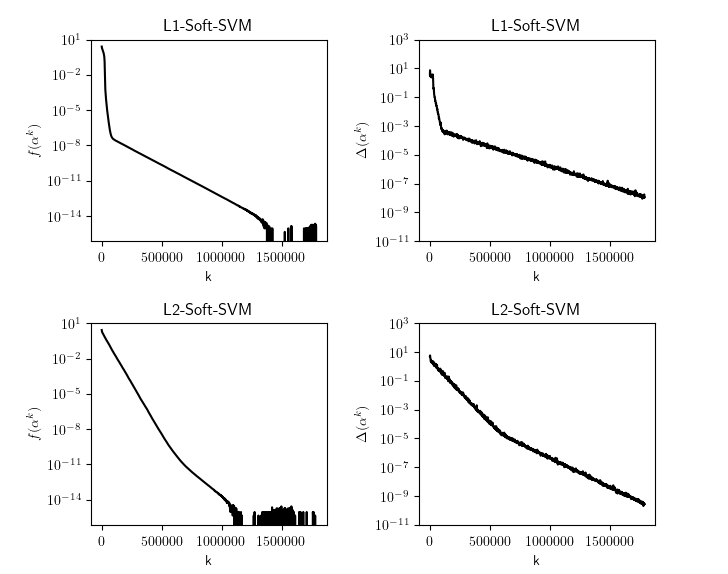
\includegraphics[scale=0.4]{abbildungen/exp-a.png}
	\caption{Konvergenzverhalten der Koordinaten-Abstiesmethode vom $L1-$ und $L2$-Soft-SVM.}
	\label{img:exp-1}
\end{figure}

Zu erkennen ist, dass die Konvergenzrate auf der linken Seite doppelt so hoch ist, wie auf der rechten. Dies geht mit der quadratischen Form der Zielfunktion einher. Weiter deutet das (im Trend) - bis auf den Knick - sehr lineare Verhalten aller Graphen auf eine lineare Konvergenz der Zielfunktion $f$ , sowie $\Delta(\alpha^k)$ hin. Die am Ende auftretenden Fluktuationen der beiden Graphen auf der linken Seite lassen sich mit der maximalen Maschinengenauigkeit von ungefähr $1.1 \cdot 10^-{16}$ erklären.

\section{Experiment B: Einfluss der randomisierten Permutation des Koordinatenabstiegs}
\begin{figure}[htbp]
	\centering
	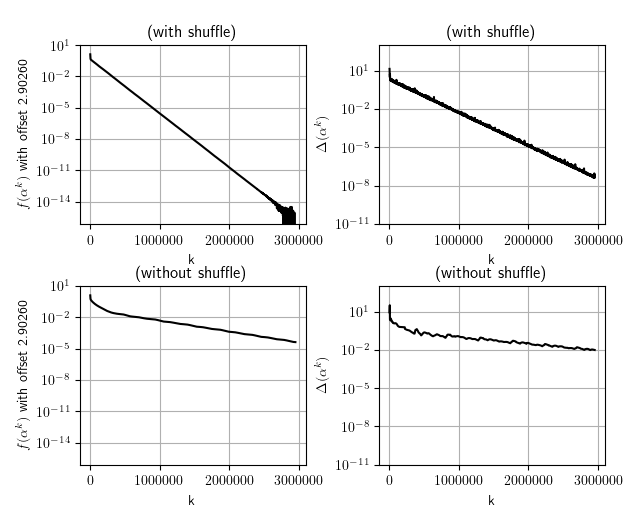
\includegraphics[scale=0.5]{abbildungen/exp-b.png}
	\caption{Konvergenzverhalten der Koordinaten-Abstiesmethode vom $L2$-Soft-SVM einmal mit und einmal ohne der Permutationen-Strategie.}
	\label{img:exp-b}
\end{figure}
Wir wollen nun den Einfluss der zufälligen Permutationen der Koordinaten in einem äußeren Zyklusdurchlauf auf die Konvergenzgeschwindigkeit untersuchen. Hierfür vergleichen wir den L2-Soft-SVM mit und ohne der Permutationen-Strategie. Für dieses Experiment wurden die Kategorien \emph{sci.electronics}, \emph{comp.sys.ibm.pc.hardware} aus dem 20newsgroup-Datenset herangezogen. Für die Parameter des L2-Soft-SVM wurden in beiden Fällen C=1, tol=$10^-9$ und max\_it=2500 gewählt.

Auf der Abbildung \ref{img:exp-b} sind 4 Plots zu erkennen. Die Plots auf der linken Seite wurden mit der Permutationen-Strategie gebildet, die beiden auf der rechten Seite ohne Permutationen-Strategie. Es ist deutlich zu erkennen, dass die Permutationen-Strategie zu einer schnelleren Konvergenz führt.

\section{Experiment C: Textklassifizierung} \label{sec:exp-c}
In diesem Experiment wird die Klassifizierungsgenauigkeitim Sinne der aus Kapitel 1 definierten Metriken, sowie der Trainingszeit für die L1-, L2-Soft-SVM, \emph{LibSVM} \cite{chang-libsvm-11}, und dem multinomialen \emph{Naive-Bayes-Verfahren} verglichen. Die LibSVM löst das duale Problem für die Hard-SVM mit Schlupfvariablen. Für die L1-, L2-Soft-SVM und  LibSVM wurden die Parameter C = 1 und tol = $10^-4$ gesetzt. er resultierende lineare Klassifizierer ordnet jedem Dokument genau eine Klasse zu. Hierfür wurde die one-vs-rest Strategie benutzt. Zu Beginn des Experimentes wurden die Dokumente in ein Trainings- und ein Test-Segment aufgeteilt. In der \emph{Trainingsphase} wurden die Modelle mit den Daten aus dem Trainingssegment erzeugt, für die \emph{Testphase} wurden dann die Trainingsdaten herangezogen. Aus Performance-Gründen wurde für den Test die von scikit-learn bereitgestellte Software \emph{Liblinear} \cite{fan-liblinear-08} und LibSVM benutzt.

\begin{table}[h!]
	\centering
	\begin{tabular}{|l | c | c |}
		\hline
		& neg. klassifiziert & pos. klassifiziert \\
		\hline 
		echt neg. & a & b \\
		\hline 
		echt pos. & c & d \\
		\hline
	\end{tabular}
	\caption{Mögliche Fälle bei einem Binärklassifikator: c stellt den Fehler 1. Art da, b den Fehler 2. Art.}
	\label{tab:fehlerarten}
\end{table}

Als Metriken für die Evaluierung wurden die \emph{Precision} (P), der \emph{Recall} (R) und der F1-Score ($F_1$)  (siehe etwa \cite{f-ir}) für die einzelnen Klassen (one vs. rest) berechnet und anschließend ihr Mittelwert gebildet. Mit der Tabelle \ref{tab:fehlerarten} ergeben sich die Precision aus dem Anteil der korrekt positiv klassifizierten zu allen positiv klassifizierten Testvektoren $(d/(b+d))$, der Recall aus dem Anteil der korrekt positiv klassifizierten zu allen echt positiven Testvektoren ($d/(c+d)$) und der F1-Score zu $F_1 = 0.5 / (P^{-1} + R^{-1})$. \\

Die Resultate zu den einzelnen Klassen wurden in den Tabellen \ref{tab:MNB}, \ref{tab:LibSVM}, \ref{tab:L1SoftSVM} und \ref{tab:L2SoftSVM} zusammengefasst. Tabelle \ref{tab:ml-avg} fasst die gemessenen Mittelwerte (average) der Precision, dem Recall und dem F1-Score, sowie Trainings- und Klassifizierungszeiten (training time/prediction time) zusammen. \\

\begin{table}[h!]
\centering
\begin{tabular}{|l | r | r | r | r| r|}
\hline
                            & precision  & recall & f1-score & train. (s) & pred. (s) \\
\hline
Multinomial Naive Bayes   	&0.76      & 0.76     & 0.74& 0.250 & 0.078 \\
LibSVM   					&0.74      & 0.73     & 0.73& 87.67 & 69.14 \\
L1-Soft-SVM (Liblinear)  &0.78      & 0.78     & 0.78& 12.49 & 0.047 \\
L2-Soft-SVM (Liblinear)  &0.79      & 0.79     & 0.78& 13.09 & 0.042 \\
\hline
\end{tabular}
\caption{Gemessene Genauigkeit, Trainings- und Klassifizierungszeit vom multinomialen Naive-Bayes, LibSVM, $L_1$-Soft-SVM und L2-Soft-SVM für den 20newsgroup-Datensatz. }
\label{tab:ml-avg}
\end{table}

Die Tabelle \ref{tab:ml-avg} zeigt, dass die Textklassifizierung mit der in der Arbeit vorgestellten Implementierung der $L_1$- und L2-Soft-SVM auch im Vergleich zu anderen Verfahren brauchbare Ergebnisse liefert. Außerdem ist erkennbar, dass die Trainingszeiten bei der $L_1$- und der L2-Soft-SVM ähnlich sind. Im Vergleich zur LibSVM sind die Trainingszeiten  deutlich geringer, im Vergleich zum multinomialen Naive-Bayes-Verfahren deutlich höher. Die Klassifizierungszeiten sind beim $L_1$- und L2 am geringsten. Die hohe Klassifizierungszeit bei der LibSVM ergibt sich dadurch, dass bei der Entscheidungsfunktion 
$$
\sign \left( \sum_{i= 1}^{l} y_i \alpha_i K(x_i,x) + b \right)
$$ 
auch im linearen Fall der Kernel $K$ für jede Trainingsinstanz einzeln berechnet wird, siehe hierzu etwa \cite{chang-libsvm-11}.
  
\chapter{Anhang: Theorie zu den restringierten Optimierungsaufgaben}
Die nächsten Definitionen sind mit ein paar wenigen Anpassungen zur Vereinfachung dem Buch \cite{gk-tnro} entnommen.

\begin{definition}[Primales Problem]
	Seien $f \in C^1(\mathbb{R}^n)$ konvex und $g_i,h_j :\mathbb{R}^n \rightarrow \mathbb{R}$ affin linear für $i=1,...m$, $j=1,...p$. Wir nennen
	\begin{equation}
	\begin{aligned}
	\min f(x) \qquad \text{u.d.N.} \qquad g_i(x) & \leq 0, i = 1,...,m \\
	h_j(x) &=0, j = 1,...,p
	\end{aligned}
	\end{equation}
	das primale Problem (P).
\end{definition}

\begin{definition}[Lagrange-Funktion]
	Die durch
	\begin{equation}
	L(x,\lambda,\mu) := f(x)+\sum_{i=1}^m \lambda_i g_i(x) + \sum_{j=1}^p \mu_i h_j(x)
	\end{equation}
	definierte Abbildung $L: \mathbb{R}^n \times \mathbb{R}^m \times \mathbb{R}^p \rightarrow \mathbb{R}$ heißt Lagrangefunktion des restringierten Optimierungsproblems $(P)$.
\end{definition}

\begin{definition}[Karush-Kuhn-Tucker]\label{def:kkt}
	Betrachte das Optimierungsproblem $(P)$.
	\begin{itemize}
		\item[(i)] Die Bedingungen
		\begin{equation}
		\begin{aligned}
		\nabla_x L(x,\lambda,\mu) &= 0,\\
		h(x) &= 0, \\
		\lambda \geq 0, g(x) \leq 0, \lambda^t g(x) &= 0
		\end{aligned}
		\end{equation}
		heißen Karush-Kuhn-Tucker-Bedingungen, oder kurz KKT-Bedingungen, des Optimierungsproblems $(P)$. Die Bedingung $\lambda^t g(x)=0$ wird auch komplementärer Schlupf genannt.
		\item[(ii)] Jeder Vektor $(x^*,\lambda^*,\mu^*) \in \mathbb{R}^n \times \mathbb{R}^m \times \mathbb{R}^p$, der den KKT-Bedingungen genügt, heißt Karush-Kuhn-Tucker-Punkt (kurz KKT-Punkt) des Optimierungsproblems $(P)$.	
	\end{itemize}
\end{definition}

\begin{definition}[Sattelpunkt]
	Ein Vektor $(x^*,\lambda^*,\mu^*) \in \mathbb{R}^n \times \mathbb{R}^m \times \mathbb{R}^p$ mit $\lambda^* \geq 0$ heißt Sattelpunkt der Lagrangefunktion $L$, wenn die Ungleichungen
	\begin{equation}
	L(x^*,\lambda,\mu) \leq L(x^*,\lambda^*,\mu^*) \leq L(x,\lambda^*,\mu^*)
	\end{equation}
	für alle $(x,\lambda,\mu) \in \mathbb{R}^n \times \mathbb{R}^m \times \mathbb{R}^p$ gelten.
\end{definition}

\begin{definition}
	Die Funktion 
	$$q(\lambda,\mu) := \inf_{x \in \mathbb{R}^n} L(x,\lambda,\mu)$$
	heißt die duale Funktion von $(P)$, das Optimierungsproblem $$
	\max{q(\lambda,\mu)} \qquad \text{u.d.N.} \qquad \lambda \geq 0, \mu \in \mathbb{R}^p$$
	das duale Problem oder Dualproblem $(D)$ zu $(P)$.
\end{definition}

\begin{satz}
	\label{dual-kkt}
	Betrachte das konvexe Optimierungsproblem $(P)$. Dann ist $x^* \in \mathbb{R}^n$ genau dann ein globales Minimum von $(P)$, wenn es Lagrange-Multiplikatoren $\lambda^* \in \mathbb{R}^m$ und $\mu^* \in \mathbb{R}^p$ gibt, sodass das Tripel $(x^*,\lambda^*,\mu^*)$ ein KKT-Punkt von $(P)$ ist.
\end{satz}
\begin{proof}
	Siehe Korollar 2.47 in \cite{gk-tnro}.
\end{proof}

Die Beweisideen des nächsten Satz stammen aus \cite{g-af-09} (Satz 5.19).
\begin{satz}
	\label{dual-satz}
	 Sei  $(x^*,\lambda^*,\mu^*) \in \mathbb{R}^n \times \mathbb{R}^m \times \mathbb{R}^p$. Dann sind äquivalent:
	\begin{itemize}
		\item[(i)] $(x^*, \lambda^*, \mu^*)$ ist ein KKT-Punkt von $(P)$
		\item[(ii)] $(x^*, \lambda^*, \mu^*)$ ist ein Sattelpunkt der zu $(P)$ zugehörigen Lagrangefunktion
		\item[(iii)] $x^*$ löst $(P)$ und $(\lambda^*, \mu^*)$ löst $(D)$
	\end{itemize}
\end{satz}
\begin{proof}
	Die Äquivalenz zwischen (i) und (ii) zeigt Korollar 2.50 (c) aus \cite{gk-tnro}. Wir zeigen die Äquivalenz von (ii) und (iii). 
	Seien 
	$$ \inf{(P)} := \inf{\{ f(x) \, | \, x \in \mathbb{R}^n ,\ g(x) \leq 0 ,\ h(x) = 0 \}},$$
	$$
	\sup{(D)} := sup{\{ q(\lambda, \mu) \lambda \geq 0 ,\ \mu \in \mathbb{R}^n \}}
	$$
	die Optimalwerte des primalen und des dualen Problems. Für $(P)$ und $(D)$ gilt nach \cite{gk-tnro} starke Dualität gilt, anders formuliert ist also $\sup{(D)} = \inf{(P)}$. \\
	
	$(iii) \Rightarrow (ii)$:
	Seien also $(x^*,\lambda^*,\mu^*)$ Lösungen für $(P)$ bzw. $(D)$. Dann gilt
	$$
	\sup(D) = \sup_{\lambda \geq 0, \mu} \inf_{x \in \mathbb{R}^n}{L(x,\lambda, \mu)} = \inf_{x \in \mathbb{R}^n} L(x, \lambda^*, \mu^*) \leq  L(x^*, \lambda^*,\mu^*) \leq \sup_{\lambda \geq 0, \mu} L(x^*, \lambda, \mu) = \inf{(P)}.
	$$
	Aus der starken Dualität folgt nun für alle Ungleichungen Gleichheit. Damit ist $$
	\sup_{\lambda \geq 0, \mu} L(x^*, \lambda, \mu) = L(x^*, \lambda^*,\mu^*) = \inf_{x \in \mathbb{R}^n} L(x, \lambda^*, \mu^*).$$
	Also ist $(x^*,\lambda^*, \mu^*)$ ein Sattelpunkt.
	
	$(iii) \Leftarrow (ii)$: Es sei nun $(x^*, \lambda^*, \mu^*)$ sein Sattelpunkt. Es gilt komplementärer Schlupf. Weiter ist 
	$$
	L(x^*,\lambda^*,\mu^*) = \inf_{x\in\mathbb{R}^n}L(x,\lambda^*,\mu^*) \leq  \sup_{\lambda \geq 0, \mu}\inf_{x\in\mathbb{R}^n}L(x,\lambda,\mu) = 
	\sup{(D)} = \inf{(P)}.
	$$
	Damit ist $L(x^*,\lambda^*,\mu^*) = f(x^*) \leq \inf{(P)}$. Also löst $x^*$ das primale Problem. Weiter ist 
	$$
	q(\lambda^*,\mu^*)=\inf_{x \in \mathbb{R}^n}{L(x,\lambda^*,\mu^*)} = L(x^*,\lambda^*,\mu^*) = f(x^*) = \inf{(P)} = \sup{(D)}.
	$$
	Damit löst $(\lambda^*, \mu^*)$ das duale Problem.	
\end{proof}

\begin{satz}
\label{satz-strict-konvex-innprdt}
	Die Funktion $\langle x, x \rangle = ||x||^2$ ist strikt konvex.
\end{satz}
\begin{proof}
	Für $||x||^2 = \langle x ,\ x \rangle$ gilt $\langle \nabla \langle x,x \rangle, h \rangle = 2 \langle x, h \rangle$. Weiter ist mit $x ,\ y \in \mathbb{R}^n$ und $x \neq y$
	$$
	\begin{aligned}
	\langle x, x \rangle - \langle y, y \rangle > 2 \langle y , x - y \rangle \Leftrightarrow
	\langle x, x \rangle + \langle y, y \rangle > 2 \langle y , x \rangle 
	\Leftrightarrow
	\langle x-y, x-y \rangle > 0 \Leftrightarrow  x \neq y.
	\end{aligned}
	$$
	Damit ist nach Satz 2.16 \cite{gk-tnro} $\langle \, . \, , \, . \, \rangle$ strikt konvex.
\end{proof}

\chapter{Anhang: Zusatzmaterial für Experiment C}
\label{chap:zusatz-exp-c}
Im folgenden sind die Tabellen aus \emph{Experiment C} aufgeführt.
\begin{table}[h!]
\centering
\begin{tabular}{|l | r | r | r | r|}
\hline
Multinomial Naive Bayes        & precision  &  recall &  f1-score &   support \\
\hline
             alt.atheism       & 0.79      & 0.73      & 0.76      & 319 \\
           comp.graphics       & 0.68      & 0.73      & 0.70      & 389 \\
 comp.os.ms-windows.misc       & 0.33      & 0.01      & 0.01      & 394 \\
comp.sys.ibm.pc.hardware       & 0.56      & 0.76      & 0.65      & 392 \\
   comp.sys.mac.hardware       & 0.85      & 0.71      & 0.77      & 385 \\
          comp.windows.x       & 0.63      & 0.85      & 0.72      & 395 \\
            misc.forsale       & 0.95      & 0.61      & 0.74      & 390 \\
               rec.autos       & 0.86      & 0.90      & 0.88      & 396 \\
         rec.motorcycles       & 0.97      & 0.90      & 0.93      & 398 \\
      rec.sport.baseball       & 0.97      & 0.85      & 0.90      & 397 \\
        rec.sport.hockey       & 0.93      & 0.96      & 0.95      & 399 \\
               sci.crypt       & 0.63      & 0.95      & 0.76      & 396 \\
         sci.electronics       & 0.79      & 0.63      & 0.70      & 393 \\
                 sci.med       & 0.86      & 0.82      & 0.84      & 396 \\
               sci.space       & 0.82      & 0.88      & 0.85      & 394 \\
  soc.religion.christian       & 0.68      & 0.96      & 0.80      & 398 \\
      talk.politics.guns       & 0.68      & 0.91      & 0.78      & 364 \\
   talk.politics.mideast       & 0.81      & 0.95      & 0.87      & 376 \\
      talk.politics.misc       & 0.58      & 0.64      & 0.60      & 310 \\
      talk.religion.misc       & 0.92      & 0.32      & 0.47      & 251 \\
\hline
               avg / total     & 0.76      & 0.76      & 0.74      & 7532 \\
\hline			 
\end{tabular}
\caption{Klassifizierungsgenauigkeit für das Multinomial-Naive-Bayes-Verfahren.}
\label{tab:MNB}
\end{table}
			 
\begin{table}[h!]
\centering
\begin{tabular}{|l | r | r | r | r|}
\hline
L2-Soft-SVM                    & precision  &  recall &  f1-score &   support \\
\hline
             alt.atheism       & 0.75      & 0.72      & 0.73      & 319  \\
           comp.graphics       & 0.67      & 0.72      & 0.69      & 389 \\
 comp.os.ms-windows.misc       & 0.71      & 0.65      & 0.68      & 394 \\
comp.sys.ibm.pc.hardware       & 0.63      & 0.67      & 0.65      & 392 \\
   comp.sys.mac.hardware       & 0.73      & 0.78      & 0.76      & 385 \\
          comp.windows.x       & 0.81      & 0.69      & 0.74      & 395 \\
            misc.forsale       & 0.80      & 0.88      & 0.84      & 390 \\
               rec.autos       & 0.84      & 0.83      & 0.84      & 396 \\
         rec.motorcycles       & 0.89      & 0.93      & 0.91      & 398 \\
      rec.sport.baseball       & 0.86      & 0.88      & 0.87      & 397 \\
        rec.sport.hockey       & 0.93      & 0.93      & 0.93      & 399 \\
               sci.crypt       & 0.89      & 0.90      & 0.89      & 396 \\
         sci.electronics       & 0.68      & 0.68      & 0.68      & 393 \\
                 sci.med       & 0.82      & 0.77      & 0.80      & 396 \\
               sci.space       & 0.88      & 0.88      & 0.88      & 394 \\
  soc.religion.christian       & 0.82      & 0.91      & 0.86      & 398 \\
      talk.politics.guns       & 0.72      & 0.84      & 0.77      & 364 \\
   talk.politics.mideast       & 0.92      & 0.79      & 0.85      & 376 \\
      talk.politics.misc       & 0.69      & 0.51      & 0.59      & 310 \\
      talk.religion.misc       & 0.61      & 0.62      & 0.62      & 251 \\
\hline
             avg / total       & 0.79      & 0.79      & 0.78      & 7532 \\
\hline			 
\end{tabular}
\caption{Klassifizierungsgenauigkeit für die L2-Soft-SVM-Machine.}
\label{tab:L2SoftSVM}
\end{table}

\begin{table}[h!]
\centering
\begin{tabular}{|l | r | r | r | r|}
\hline
L1-Soft-SVM                    & precision  &  recall &  f1-score &   support \\
\hline
             alt.atheism       & 0.75      & 0.72      & 0.74      & 319  \\
           comp.graphics       & 0.68      & 0.71      & 0.69      & 389 \\
 comp.os.ms-windows.misc       & 0.69      & 0.66      & 0.68      & 394 \\
comp.sys.ibm.pc.hardware       & 0.62      & 0.66      & 0.64      & 392 \\
   comp.sys.mac.hardware       & 0.73      & 0.78      & 0.75      & 385 \\
          comp.windows.x       & 0.80      & 0.68      & 0.74      & 395 \\
            misc.forsale       & 0.79      & 0.86      & 0.83      & 390 \\
               rec.autos       & 0.83      & 0.83      & 0.83      & 396 \\
         rec.motorcycles       & 0.90      & 0.93      & 0.91      & 398 \\
      rec.sport.baseball       & 0.84      & 0.88      & 0.86      & 397 \\
        rec.sport.hockey       & 0.93      & 0.93      & 0.93      & 399 \\
               sci.crypt       & 0.89      & 0.90      & 0.89      & 396 \\
         sci.electronics       & 0.67      & 0.68      & 0.68      & 393 \\
                 sci.med       & 0.82      & 0.77      & 0.80      & 396 \\
               sci.space       & 0.89      & 0.88      & 0.89      & 394 \\
  soc.religion.christian       & 0.82      & 0.91      & 0.86      & 398 \\
      talk.politics.guns       & 0.72      & 0.83      & 0.77      & 364 \\
   talk.politics.mideast       & 0.92      & 0.79      & 0.85      & 376 \\
      talk.politics.misc       & 0.70      & 0.51      & 0.59      & 310 \\
      talk.religion.misc       & 0.61      & 0.62      & 0.61      & 251 \\
\hline
             avg / total      & 0.78      &  0.78     & 0.78      & 7532\\
\hline			 
\end{tabular}
\caption{Klassifizierungsgenauigkeit für die L1-Soft-SVM-Machine.}
\label{tab:L1SoftSVM}
\end{table}

\begin{table}[h!]
\centering
\begin{tabular}{|l | r | r | r | r|}
\hline
LibSVM                         & precision  &  recall &  f1-score &   support \\
\hline
             alt.atheism       & 0.67      & 0.68      & 0.68      & 319  \\
           comp.graphics       & 0.60      & 0.72      & 0.65      & 389 \\
 comp.os.ms-windows.misc       & 0.68      & 0.63      & 0.66      & 394 \\
comp.sys.ibm.pc.hardware       & 0.61      & 0.65      & 0.63      & 392 \\
   comp.sys.mac.hardware       & 0.69      & 0.71      & 0.70      & 385 \\
          comp.windows.x       & 0.80      & 0.66      & 0.72      & 395 \\
            misc.forsale       & 0.80      & 0.87      & 0.83      & 390 \\
               rec.autos       & 0.74      & 0.79      & 0.76      & 396 \\
         rec.motorcycles       & 0.84      & 0.85      & 0.85      & 398 \\
      rec.sport.baseball       & 0.77      & 0.76      & 0.76      & 397 \\
        rec.sport.hockey       & 0.90      & 0.85      & 0.88      & 399 \\
               sci.crypt       & 0.83      & 0.84      & 0.84      & 396 \\
         sci.electronics       & 0.65      & 0.66      & 0.65      & 393 \\
                 sci.med       & 0.67      & 0.63      & 0.65      & 396 \\
               sci.space       & 0.89      & 0.81      & 0.85      & 394 \\
  soc.religion.christian       & 0.82      & 0.89      & 0.85      & 398 \\
      talk.politics.guns       & 0.65      & 0.79      & 0.72      & 364 \\
   talk.politics.mideast       & 0.91      & 0.72      & 0.80      & 376 \\
      talk.politics.misc       & 0.59      & 0.46      & 0.52      & 310 \\
      talk.religion.misc       & 0.53      & 0.57      & 0.55      & 251 \\
\hline
              avg / total      & 0.74      & 0.73      & 0.73      &7532 \\
\hline			 
\end{tabular}
\caption{Klassifizierungsgenauigkeit für die LibSVM (Hard-SVM mit Schlupfvariablen).}
\label{tab:LibSVM}
\end{table}

\chapter{Anhang: Programmcode für die Experimente}
Folgender Programmcode wurde für die Experimente benutzt:
\lstinputlisting[language=Python,caption=svm.py,label=lst:svm]{exp/svm.py}
\lstinputlisting[language=Python,caption=exp-a.py,label=lst:exp-a]{exp/exp-a.py}
\lstinputlisting[language=Python,caption=exp-b.py,label=lst:exp-b]{exp/exp-b.py}
\lstinputlisting[language=Python,caption=exp-c.py,label=lst:exp-c]{exp/exp-c.py}
\lstinputlisting[language=Python,caption=exputils.py,label=lst:exputils]{exp/exputils.py}



%%%%%%%%%%%%%%%%%%%%%%%%%%%%%%%%%%%%%%%%%%%%%%%%%%%%%%%%%%%%%%%%%%%%%%%%%%%%%%%%
\thesisbibliography
\bibliography{mybib}


\appendix


%\clearpage
%\pdfbookmark[0]{ToDo-Liste}{todos}
%\listoftodos

\end{document}
